%%%%%%%%%%%%%%%%%%%%%%%%%%%%%%%%%%%%%%%%
%% HiMCM/MidMCM LaTeX Template -- 2026 %%
%% CP-SET Framework -- complete five-task manuscript
%% Efficiency/effectiveness scope separation, November 8, 2026.
%%%%%%%%%%%%%%%%%%%%%%%%%%%%%%%%%%%%%%%%
\documentclass[12pt]{article}
\usepackage{geometry}
\geometry{left=1in,right=0.75in,top=1in,bottom=1in}
\newcommand{\Problem}{B}
\newcommand{\Team}{18588}
\usepackage{newtxtext}
\usepackage{amsmath,amssymb,amsthm}
\usepackage{newtxmath}
\usepackage[pdftex]{graphicx}
\usepackage{xcolor}
\usepackage{fancyhdr}
\usepackage{microtype}
\usepackage{xurl}
\usepackage{needspace}
\usepackage{booktabs,tabularx,array}
\usepackage{enumitem,titlesec,caption,multicol,tocloft,float,placeins}
\usepackage[hidelinks]{hyperref}
\newif\ifinlineai
\inlineaitrue
\captionsetup{font=small,labelfont=bf,skip=4pt}
\titlespacing*{\section}{0pt}{10pt plus2pt minus1pt}{5pt}
\titlespacing*{\subsection}{0pt}{8pt plus1pt minus1pt}{3pt}
\setlength{\textfloatsep}{9pt plus2pt minus2pt}
\setlength{\floatsep}{7pt plus1pt minus1pt}
\setlength{\intextsep}{8pt plus1pt minus1pt}
\setcounter{topnumber}{5}
\setcounter{bottomnumber}{4}
\setcounter{totalnumber}{8}
\renewcommand{\topfraction}{.95}
\renewcommand{\bottomfraction}{.9}
\renewcommand{\textfraction}{.05}
\renewcommand{\floatpagefraction}{.85}
\setlength{\headheight}{15pt}
\setlength{\parskip}{1.5pt}
\setlength{\parindent}{1.2em}
\widowpenalty=10000
\clubpenalty=10000
\lhead{Team \Team}
\rhead{}
\cfoot{}
\newtheorem{theorem}{Theorem}
\newtheorem{corollary}[theorem]{Corollary}
\newtheorem{lemma}[theorem]{Lemma}
\newtheorem{definition}{Definition}

\begin{document}
\graphicspath{{.}}
\DeclareGraphicsExtensions{.pdf,.jpg,.png}
\thispagestyle{empty}
\vspace*{-16ex}
\centerline{\begin{tabular}{*3{c}}
\parbox[t]{0.3\linewidth}{\begin{center}\textbf{Problem Chosen}\\ \Large \Problem\end{center}}&
\parbox[t]{0.3\linewidth}{\begin{center}\textbf{2026\\ HiMCM/MidMCM\\ Summary Sheet}\end{center}}&
\parbox[t]{0.3\linewidth}{\begin{center}\textbf{Team Control Number}\\ \Large \Team\end{center}}\\
\hline
\end{tabular}}

\begin{center}
\vspace{1.1em}
{\Large\bfseries CP-SET: Measuring Useful Cooling\\in Open Public Spaces}\\[.5em]
{\bfseries Summary}
\end{center}
An open cooling system should be judged by the useful service reaching its users. We develop the \textbf{Coupled Psychrometric-SET Service Efficiency \& Effectiveness Framework (CP-SET)} to connect heat and moisture balances, local air delivery, human thermal response and operational decisions.

The freezer case establishes four essential quantities: service quantity, local quality, duration and electrical input. Its useful storage service motivates a human-service analogue: signed SET-excess relief accumulated over passenger-hours, divided by the electricity used by every operating device. This distinguishes efficiency from the adequacy of the cooling delivered.

For a New York City bus-shelter geometry, the framework combines wet-bulb-limited evaporation, dry-air-weighted local mixing and Standard Effective Temperature. At $34^\circ$C, fan A achieves efficiencies of $84.58$ and $90.57$ person$\cdot{}^\circ$C$\cdot$h/kWh at $30\%$ and $70\%$ RH. B and C require $4.8$ and $10$ times A's accumulated relief to overcome their power ratios. A delivery-loss test identifies where B overtakes A. A separate hot-dry test shows why larger thermal improvement need not imply higher efficiency.

At Canberra MRT station, the same delivery and response modules are retained while zone enthalpy, humidity and surface temperature evolve with exchange, passenger loads and equipment operation. Across 24 sampled installations, A3 reaches the highest efficiency, $37.58$; among six equal-coverage benchmarks, A36 leads at $35.49$. Relocating the same AB30 inventory toward passenger demand raises its efficiency from $15.39$ to $18.39$. Coverage and local delivery therefore matter alongside the rated cooling effect.

At Ullman Terrace, Phoenix, and Satay Street, Singapore, we enumerate integer layouts and compare pure devices at equal coverage. The B--C efficiency order reverses between dry and humid climates. Adding thermal, access and annual-energy requirements yields different cost-minimizing plans: \textbf{A10C2 in Phoenix} provides $1248.87$ service units using $30$ kWh per four-hour session; \textbf{A10 in Singapore} provides $971.22$ using $10$ kWh. Their equivalent annual costs are USD $3360$ and $1293$ under the common planning prices. The Phoenix choice persists in $93.8\%$ of tested price combinations; Singapore's persists in all of them.

Conservation checks, limiting-case recovery and time-step refinement verify the numerical implementation. Climate, local delivery and cost sensitivities identify the assumptions that affect the decision. The resulting memorandum and public explanation translate useful cooling per kWh into equipment placement, operating schedules and extreme-heat procedures.

\noindent\textbf{Keywords:} psychrometrics; local air delivery; Standard Effective Temperature; cooling service efficiency; multi-objective decisions.

\newpage
\pagestyle{fancy}\rhead{Page \thepage}
\setcounter{tocdepth}{1}
\section*{Contents}
{\fontsize{10}{11.5}\selectfont
\setlength{\cftbeforesecskip}{1pt}
\begin{multicols}{2}
\makeatletter\@starttoc{toc}\makeatother
\end{multicols}}
\vspace{4pt}
\section{Introduction}
\label{sec:introduction}
\subsection{Background}
Open cooling systems must deliver relief despite continuous exchange with their surroundings. Fans alter human convective and evaporative losses; evaporative coolers also change air temperature and moisture \cite{fanguide,evapequip}. Comparing them requires useful service per unit energy.

\subsection{Problem Restatement}
The five tasks are to define cooling efficiency, develop bus and rail models, test two contrasting venues, extend efficiency into an effectiveness decision, and communicate operating guidance through a memorandum and public blog \cite{problem}.

\subsection{Our Modeling Framework}
Our \textbf{CP-SET Framework (Coupled Psychrometric-SET Service Efficiency \& Effectiveness Framework)} connects conserved heat and moisture to local exposure, then converts SET relief into person-time service per kWh. Requirements 1--3 compare efficiency; Requirement 4 adds cooling adequacy, visitor experience and cost. The workflow below preserves this progression.
\begin{center}
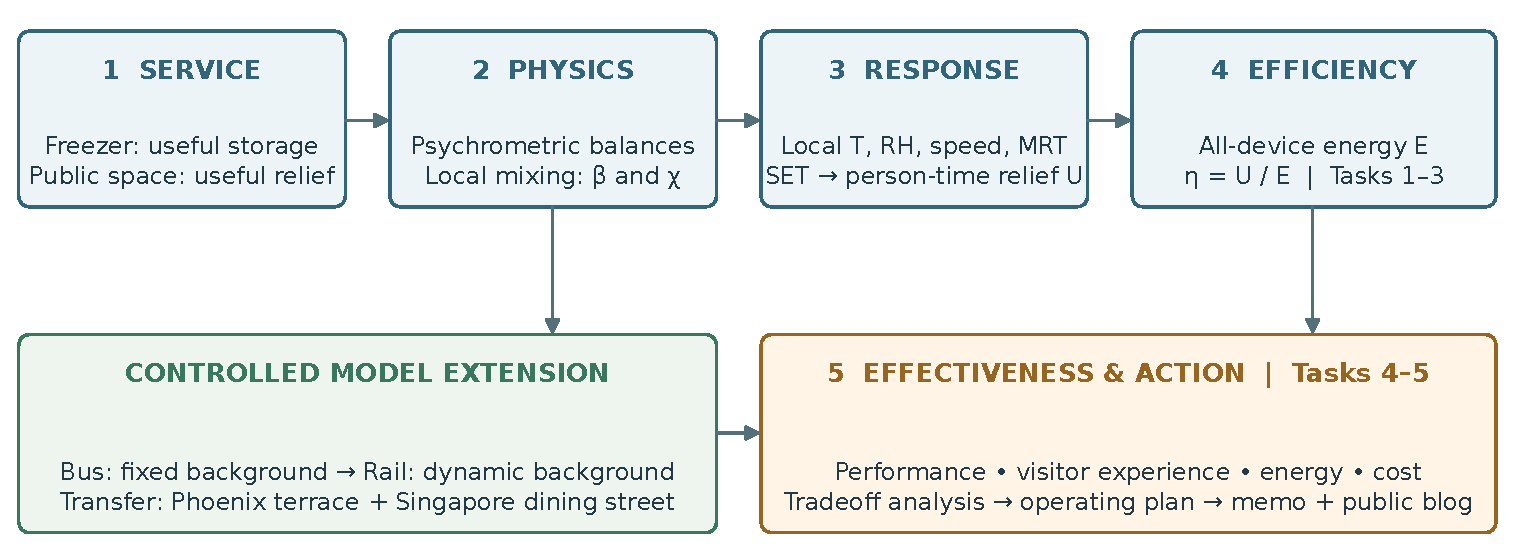
\includegraphics[width=\linewidth]{figures/29_cp_set_framework.pdf}\\[-2pt]
{\small\textbf{CP-SET workflow.} A shared physical and service model supports progressively broader decisions.}
\end{center}
\ifinlineai
\noindent\footnotesize AI assistance in model development, coding and writing is documented in the appended report \cite{codex,gemini}.\normalsize
\fi
\clearpage
\section{Assumptions and Justifications}
\begingroup\setlength{\intextsep}{4pt}
\label{sec:assumptions}
\begin{enumerate}[leftmargin=*,itemsep=2pt,topsep=2pt,label=\textbf{A\arabic*.}]
\item \textbf{Matched service boundary.} Comparisons share weather, people, geometry and period; the problem's kW/hr entries are interpreted as kW. \textit{Justification:} A common workload and complete device-energy accounting isolate strategy efficiency.
\item \textbf{Zoned air and rapid local mixing.} Zones have uniform background states; local supply mixes at negligible storage, with disjoint footprints and separately prescribed speed. \textit{Justification:} This resolves occupied-location differences when local residence time is short relative to the 120-s station disturbance.
\item \textbf{Conserved heat and water.} Evaporation is near-adiabatic; background dry-air mass is fixed and exchange is balanced; shaded radiation uses mean radiant temperature. Condensation is excluded in public-space cases. \textit{Justification:} These approximations retain the dominant transfers while counting every electrical and vapor-enthalpy source once.
\item \textbf{Reference human response.} SET uses standing transport users and seated diners at 1.2 met and 0.5 clo, with a $26^\circ$C excess reference. \textit{Justification:} One signed-relief measure compares airflow and evaporation. Dry-heat tests use $T_a=T_r=39/40^\circ$C and RH $15/20\%$: $40^\circ$C is the implementation boundary; the interior $39^\circ$C test retains the ranking \cite{pythermal}.
\item \textbf{Explicit design inputs.} Published sources establish site geometry and climate context; tabulated estimates specify operating and economic conditions. \textit{Justification:} Reproducible inputs support sensitivity analysis. Costs use one currency and horizon; equipment clearance is the visitor-access proxy. SET relief and operational heat-safety procedures serve separate purposes.
\end{enumerate}


\begin{table}[H]
\centering\fontsize{9.5}{10.7}\selectfont
\caption{Transport-case inputs. Geometry sources are cited; remaining entries are model design assumptions.}
\label{tab:bus-assumptions}\label{tab:rail-inputs}
\begin{tabularx}{\linewidth}{@{}p{.18\linewidth}XX@{}}
\toprule
Input & Bus shelter & Canberra waiting area\\
\midrule
Geometry & $4.2672\times1.5240\times2.7178$ m \cite{nycshelter}; three equal gross strips & $L=220$ m \cite{canberra-dimensions}; effective waiting width $6$ m, usable fraction $.8$, air height $4$ m; three zones\\
Climate / radiation & $T_a=34^\circ$C; RH $30/70\%$; $T_r=36^\circ$C & $T_o=33^\circ$C, RH $70\%$; external $T_{r,o}=33^\circ$C \cite{singapore-climate}\\
People / time & $(4,4,4)$ people, 1 h; redistribution $(8,3,1)$ or $(1,3,8)$ & $(26.4,44,17.6)\to(88,198,66)$ linearly per 15-min cycle; 2-h warm-up + 2-h evaluation\\
Exchange & Fixed outdoor background & ACH $(8,4,10)$ plus $(8,4,12)$ in last 2 min; adjacent flow $.88$ kg dry air/s\\
Surface / people & Prescribed radiant conditions & Per zone $C_m=17.6$ MJ/K; $H_{ma}/H_{mo}=880/1760$ W/K; absorbed load $3520$ W; $F=(.55,.85,.55)$; per person $q_c/q_r=45/30$ W, $g=45/(2.45\times10^6)$ kg/s\\
Device delivery & Profiles in Table~\ref{tab:bus-fields}; $\chi=0$; $\chi$ sensitivity uses A $\beta=(.8,.45,.1)$ and rail flows & $\beta=.5$, $\chi=1$; A/B/C flow $.6/.6/1.2$ kg dry air/s; footprints $20/30/40$ m$^2$\\
Shared response & \multicolumn{2}{p{.77\linewidth}@{}}{Pressure $101325$ Pa; $v_0=.2$ m/s; body area $1.8258$ m$^2$, external work zero; $\varepsilon_{B/C}=.7$; outlet drops capped at $5/8^\circ$C. $\Theta_c$ sensitivity $24/26/28^\circ$C.}\\
\bottomrule
\end{tabularx}
\end{table}
\begin{table}[H]
\centering\fontsize{9.5}{10.7}\selectfont
\caption{Local speed and mixing profiles in zone order; each entry describes an independent local state.}
\label{tab:bus-fields}
\begin{tabular}{@{}lccc@{}}
\toprule
Device & Bus speed (m/s) & Bus $\beta_{s,z}$ & Rail covered speed (m/s)\\
\midrule
A & $1/.55/.25$ & Immaterial at $\chi=0$ & $.60/1/.50$\\
B & $.80/.50/.30$ & $.80/.45/.10$ & $.50/.80/.45$\\
C & $1/.80/.50$ & $.90/.70/.40$ & $.75/1/.60$\\
\bottomrule
\end{tabular}
\end{table}

\endgroup
\clearpage
\IfFileExists{sections/venue_assumptions.tex}{\begin{table}[H]
\centering\fontsize{9.5}{10.7}\selectfont
\caption{Dining-venue design assumptions. Official sources establish venue identity and climate class; numerical inputs are planning estimates. Complete inputs are in \texttt{venue\_model/inputs.json}.}
\label{tab:venue-inputs}
\begin{tabularx}{\linewidth}{@{}p{.20\linewidth}XX@{}}
\toprule
Scenario input & Ullman Terrace, Phoenix & Satay Street, Singapore\\
\midrule
Venue/sector & Outdoor patio \cite{ullman}; $300$ m$^2$ in three equal zones & Open-air dining street \cite{satay-street}; $240$ m$^2$ in three equal zones\\
Climate/guests & $T_a/T_r=36/38^\circ$C, RH $25\%$; $n=(60,40,20)$ \cite{phoenix-climate} & $T_a/T_r=32/34^\circ$C, RH $75\%$; $n=(60,36,24)$ \cite{singapore-climate}\\
Delivery/response & \multicolumn{2}{p{.77\linewidth}@{}}{Fixed background, $\chi=0$; seated guests with shared met/clo/$v_0$; equal person fractions in three local strips using Table~\ref{tab:bus-fields}'s bus profiles. Zone density uniform; footprints disjoint.}\\
Unit A/B/C inputs & \multicolumn{2}{p{.77\linewidth}@{}}{$a_k=20/30/40$ m$^2$; supply $1.2/2/3$ kg dry air/s; clearance $b_k=.5/1/1.5$ m$^2$; capital USD $300/1000/2000$; annual maintenance USD $30/100/200$.}\\
Time and prices & \multicolumn{2}{p{.77\linewidth}@{}}{$H=4$ h/session, $H_y=600$ h/year; life $L=5$ y, $r=5\%$, zero salvage; USD $.20$/kWh and $3$/m$^3$; water multiplier $\lambda_w=1.15$, $\rho_w=1000$ kg/m$^3$.}\\
Task 4 limits & $\overline R_{\max}=4.5^\circ$C; $E_{\max}=6000$ kWh/y & $\overline R_{\max}=7.5^\circ$C; $E_{\max}=2400$ kWh/y\\
Comparison/policy & \multicolumn{2}{p{.77\linewidth}@{}}{Task 3 has no coverage constraint; its common-coverage benchmark uses $q=.60$. Task 4 minimizes annual cost with $q\ge.80$, $X\le.035$ and the limits above.}\\
Sensitivity & \multicolumn{2}{p{.77\linewidth}@{}}{Capital $\pm30\%$; water/electricity $\pm50\%$; RH $\pm10$ pp; evaporative $\beta\pm.15$ clipped to $[0,1]$; induced speed $\pm20\%$.}\\
\bottomrule
\end{tabularx}
\end{table}

}{}
\section{Nomenclature}
\label{sec:nomenclature}
\begin{table}[H]
\centering\fontsize{9.5}{11}\selectfont
\begin{tabularx}{\linewidth}{@{}lXl@{\hspace{9pt}}lXl@{}}
\toprule
Symbol & Meaning & Unit & Symbol & Meaning & Unit\\
\midrule
$h$ & Moist-air enthalpy & J/kg$_{da}$ & $w$ & Humidity ratio & kg/kg$_{da}$\\
$\beta_{s,z}$ & Supply dry-air mixing fraction & 1 & $\chi$ & Pre-delivery electrical heat fraction & 1\\
$T,T_r$ & Air / mean radiant temperature & $^\circ$C & $\phi$ & Relative humidity & 1\\
$\Theta,\Theta_c$ & SET / service reference & $^\circ$C & $D$ & Excess SET above $\Theta_c$ & $^\circ$C\\
$U_s$ & Accumulated useful relief & person$\cdot^\circ$C$\cdot$h & $R_s$ & Accumulated residual excess & person$\cdot^\circ$C$\cdot$h\\
$E_s$ & Electrical energy & kWh & $\eta_s$ & Cooling service efficiency & person$\cdot^\circ$C$\cdot$h/kWh\\
$c_{zk}$ & Direct-coverage fraction & 1 & $x_{zk}$ & Device count by zone/type & unit\\
$n_z$ & Mean simultaneous occupants & person & $\dot m_k$ & Dry-air supply flow & kg$_{da}$/s\\
$M_z$ & Zone dry-air mass & kg$_{da}$ & $p_k,P_k$ & Device electric power & kW, W\\
$\overline R_s$ & Mean residual SET excess & $^\circ$C & $X_s,C_{s,y}$ & Access footprint / annual cost & 1, USD/year\\
\bottomrule
\end{tabularx}
\end{table}
\noindent\small Subscripts: $s$ = candidate scheme, $z$ = zone, $k$ = device type (time interval in discrete bus sums), $0$ = matched no-cooling baseline, $b$ = background, $\ell$ = local exposure. Food service uses kg$\cdot$h/kWh; human service uses the units above.\normalsize

\clearpage
% Requirements 1 and 2(a); numbered equations retain their original order.
\section[Freezer: service efficiency]{Understanding Cooling Efficiency}
\label{sec:understand}

An open freezer succeeds by preserving food, not simply by removing heat. Low electricity use can accompany inadequate storage, while large cooling loads may reflect infiltration through the opening. We therefore evaluate \emph{useful service per unit energy}.

\begin{figure}[!ht]
\centering
\begin{minipage}[c]{0.48\linewidth}
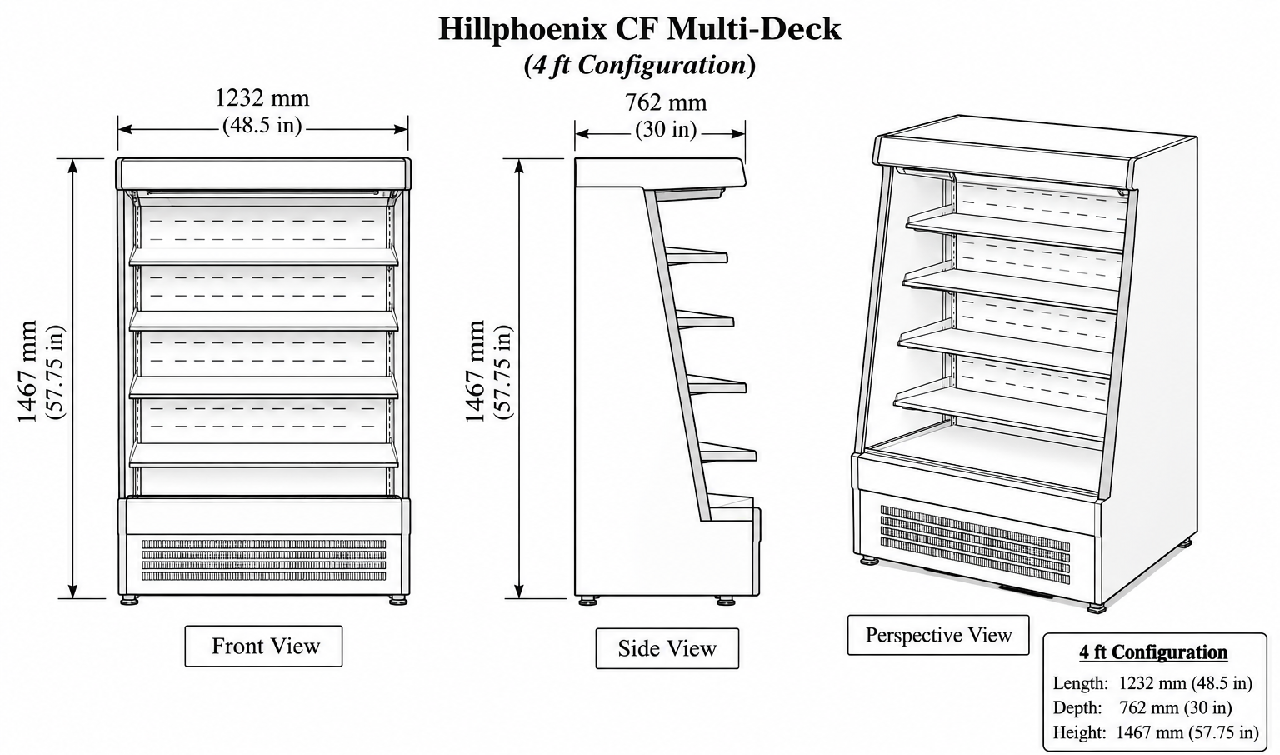
\includegraphics[width=\linewidth]{figures/09_open_display_case.pdf}
\end{minipage}\hfill
\begin{minipage}[c]{0.48\linewidth}
\small
The open front admits warm, moist air; cabinet surfaces conduct and radiate heat. Lights, fans, restocking and defrost add operating loads. Insulation and equipment condition modify these mechanisms; equipment age is not a separate score \cite{ashrae}. Product temperatures must be checked across shelves, since a mean can conceal a warm location \cite{etl}.
\end{minipage}
\caption{Open-case heat pathways and product locations. The supplied medium-temperature display schematic illustrates geometry; freezer limits remain product-specific \cite{hillphoenix}.}
\label{fig:open-case}
\end{figure}

The numerator needs \textbf{quantity, local quality and duration}: compliant product mass integrated over storage time. The denominator includes refrigeration and auxiliaries without overlapping meter readings. Matched loading, ambient conditions and complete operating cycles prevent short operation or stored cold from inflating efficiency:
\begin{equation}
\boxed{\text{Cooling efficiency}
=\frac{\text{useful service accumulated over objects and time}}
{\text{energy input over the same period}}.}
\label{eq:principle}
\end{equation}
\begin{equation}
 \eta_f=\frac{\int\sum_i m_i(t)\mathbf{1}\{T_{p,i}(t)\in\mathcal T_i\}\,dt}
 {\int p_f(t)\,dt},
\label{eq:freezer-service}
\end{equation}
Here $m_i$ is product mass (kg), $\mathcal T_i$ its admissible temperature range, $t$ is hours and $p_f$ is kW; thus $\eta_f$ is compliant kg$\cdot$h/kWh. For people, the response changes to thermal-discomfort relief weighted by occupied time. These recipient-specific numerators cannot be directly compared numerically.

\subsection{A shared physical structure}
For dry-air mass $M_z$ (kg), balanced dry-air streams $\dot m_{jz}$ (kg/s), enthalpy $h$ (J/kg dry air) and humidity ratio $w$ (kg vapor/kg dry air),
\begin{align}
 M_z\dot h_z&=\sum_j\dot m_{jz}(h_j-h_z)+S_{h,z},\\
 M_z\dot w_z&=\sum_j\dot m_{jz}(w_j-w_z)+S_{w,z}.
\label{eq:common-balance}
\end{align}
$S_h$ (W) and $S_w$ (kg/s) contain the appropriate device, occupant, product and surface sources. Freezer refrigeration can remove heat and condensate; public cooling changes airflow and moisture. The bus fixes the background and solves local delivery; the station retains that calculation while resolving background and surface storage \cite{epzone}. Figure~\ref{fig:inheritance} shows this progression. Cruz-Salas et al.\ motivate separating treatment, transport and occupied-space conditions \cite{cruz2026}.

\begin{figure}[!ht]
\centering
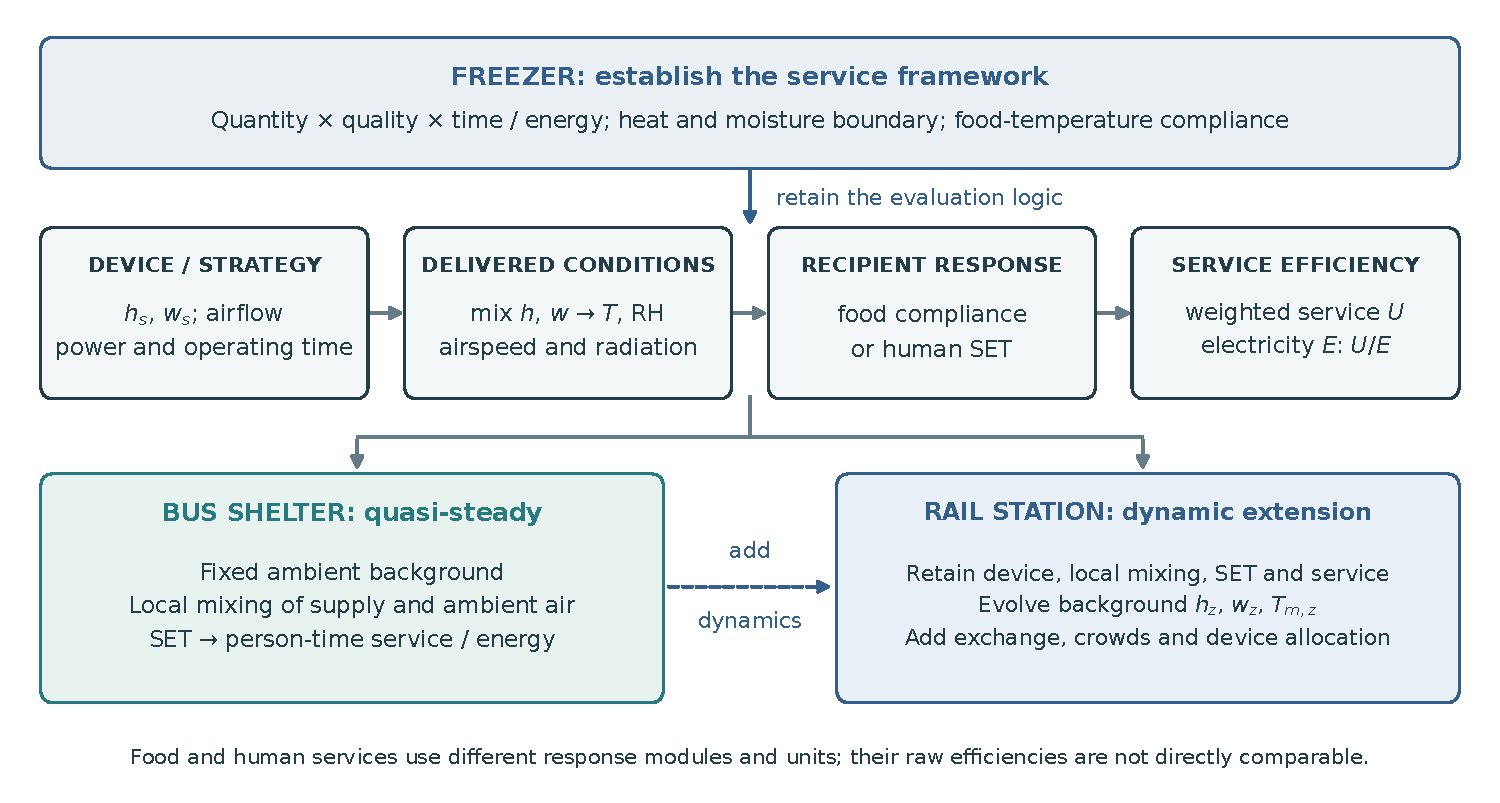
\includegraphics[width=0.94\linewidth]{figures/19_model_inheritance.pdf}
\caption{Shared conservation and service accounting, with recipient-specific response and increasingly resolved background dynamics.}
\label{fig:inheritance}
\end{figure}

\section[Bus shelter]{Bus Stop: Local Delivery and Cooling Efficiency}
\label{sec:bus}

\subsection{Geometry and comparison inputs}
NYC DOT's regular shelter measures $14$ ft by $5$ ft by $8$ ft $11$ in, or $4.2672\times1.5240\times2.7178$ m \cite{nycshelter}. Its gross footprint is $A=6.5032\,\mathrm{m^2}$. Three equal strips have $A_z=2.1677\,\mathrm{m^2}$ and centers $(x_z,W/2)$, $x_z=(z-\tfrac12)L/3$; delivery originates at $x=0$.

\begin{figure}[!ht]
\centering
\begin{minipage}[t]{0.49\linewidth}
\centering
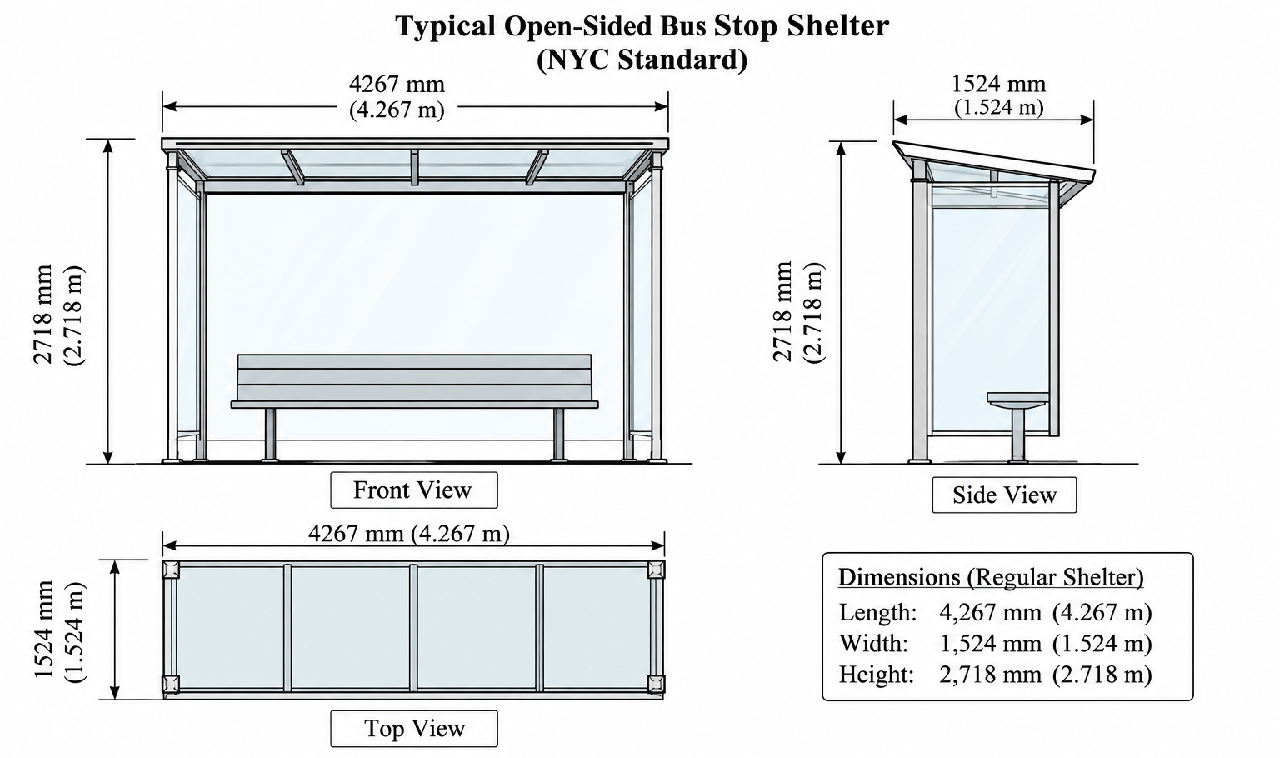
\includegraphics[width=\linewidth]{figures/07_bus_shelter_geometry.pdf}
\caption{Adopted NYC shelter dimensions \cite{nycshelter}.}
\label{fig:shelter-geometry}
\end{minipage}\hfill
\begin{minipage}[t]{0.49\linewidth}
\centering
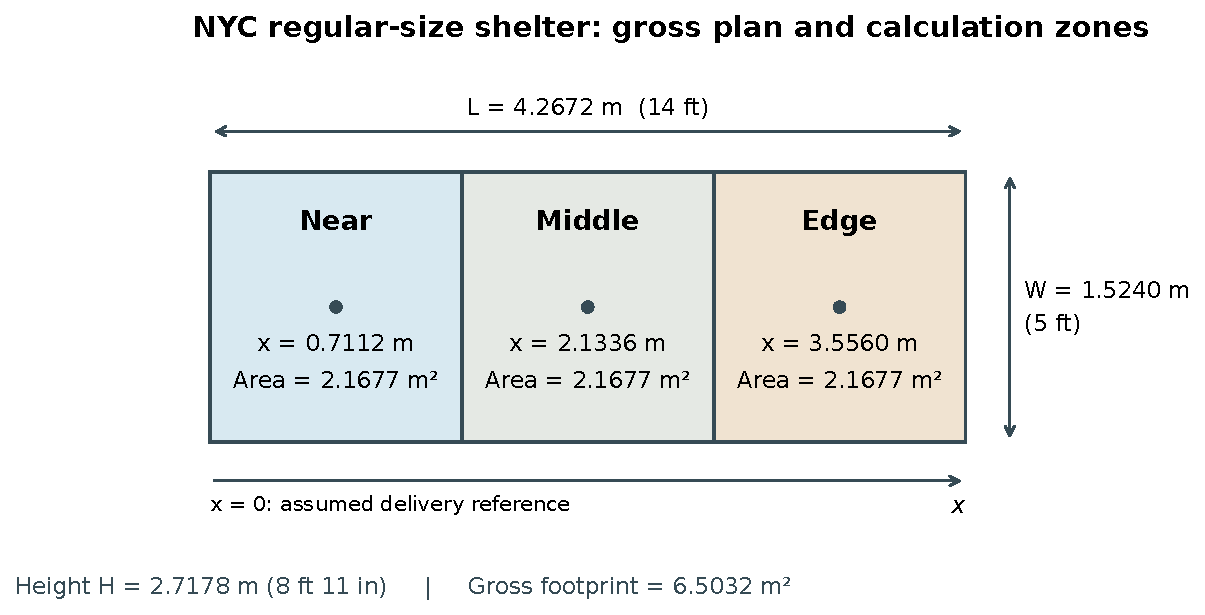
\includegraphics[width=\linewidth]{figures/08_shelter_zoning.pdf}
\caption{Equal near/middle/edge accounting strips.}
\label{fig:shelter-zones}
\end{minipage}
\end{figure}

The problem's $3\,^{\circ}\mathrm C$ fan effect describes perceived cooling; B/C's $5/8\,^{\circ}\mathrm C$ describe air cooling \cite{problem}. We interpret the listed kW/hr numbers as powers $p_{A/B/C}=0.25/1.2/2.5$ kW. Tables~\ref{tab:bus-assumptions}--\ref{tab:bus-fields} specify the comparison: $34\,^{\circ}\mathrm C$, RH $30/70\%$, $T_r=36\,^{\circ}\mathrm C$ and 12 mean occupants. Geometry enters once through $n_z=\rho_zA_z$ when density replaces headcount.

\subsection{From device outlet to occupied air}
A changes prescribed local speed while retaining background temperature and moisture in the zero-local-heat base case \cite{fanguide}. For B/C, wet-bulb temperature bounds evaporation \cite{evapequip}:
\begin{equation}
 T_{o,s}=T_b-\min\{\Delta T_s^{\max},\;\varepsilon_s(T_b-T_{wb,b})\},
 \qquad s\in\{B,C\},
\label{eq:outlet}
\end{equation}
$b$ denotes the inlet background; $\varepsilon_s$ is evaporative effectiveness and $\Delta T_{B/C}^{\max}=5/8\,^{\circ}\mathrm C$ are the adopted outlet caps. With $\phi$ as RH fraction and pressures in Pa, SI psychrometrics give \cite{psychrolib}
\begin{align}
 w&=0.621945\frac{p_v}{p-p_v},\qquad p_v=\phi p_{sat}(T),\\
 h(T,w)&=1006T+w(2501000+1860T),
\label{eq:enthalpy}
\end{align}
Temperatures are in $^{\circ}$C. The near-isenthalpic evaporative stage, $h_{o,s}\simeq h_b$, yields
\begin{equation}
 w_{o,s}=\frac{h_b-1006T_{o,s}}{2501000+1860T_{o,s}}.
\end{equation}
This stage precedes electrical heating and neglects make-up-water enthalpy \cite{evap}. A device supply mixes with entrained background in a negligible-storage local region. For $x\in\{h,w\}$,
\begin{equation}
 0=\dot m_{s,z}(x_s^{\rm sup}-x_{\ell,s,z})+
 \dot m_{e,z}(x_b-x_{\ell,s,z}),\qquad
 \beta_{s,z}=\frac{\dot m_{s,z}}{\dot m_{s,z}+\dot m_{e,z}}.
\label{eq:delivery-balance}
\end{equation}
$\beta$ is a dry-air flow fraction, not a fraction of passengers or total flow assigned to a strip. A fraction $\chi$ of unit electric power $P_s=1000p_s$ W heats unit supply flow $\dot m_s$ before reaching people:
\begin{equation}
 h_s^{\rm sup}=h_{o,s}+\chi P_s/\dot m_s,\qquad
 w_s^{\rm sup}=w_{o,s},\qquad 0\leq\chi\leq1.
\label{eq:supply-heat}
\end{equation}
For A, the unheated outlet equals the inlet. Mixing conserves $h,w$, after which temperature and RH are recovered:
\begin{align}
 w_{\ell,s,z}&=(1-\beta_{s,z})w_b+\beta_{s,z}w_s^{\rm sup},\\
 h_{\ell,s,z}&=(1-\beta_{s,z})h_b+\beta_{s,z}h_s^{\rm sup},\\
 T_{\ell,s,z}&=\frac{h_{\ell,s,z}-2501000w_{\ell,s,z}}{1006+1860w_{\ell,s,z}}.
\label{eq:mixing}
\end{align}
RH is not averaged directly. The bus uses $b=a$ and $\chi=0$. Its B/C fractions imply entrainment-to-supply ratios $(1-\beta)/\beta=0.25/1.22/9.00$ and $0.11/0.43/1.50$. Parallel strip branches share one device's total supply.

\subsection{A common response and efficiency measure}
Standard effective temperature (SET) combines air temperature, radiation, airspeed and humidity for the reference passenger \cite{thermalcomfort,pythermal}:
\begin{equation}
 \Theta_{s,z}=F_{\mathrm{SET}}(T_{\ell,s,z},T_{r,z},v_{s,z},\phi_{\ell,s,z};\mathrm{met},\mathrm{clo}).
\label{eq:set}
\end{equation}
For the assumed hot-discomfort reference $\Theta_c=26\,^{\circ}\mathrm C$, define
\begin{equation}
 D(\Theta)=[\Theta-\Theta_c]_+,\qquad [x]_+=\max(x,0).
\end{equation}
Against the same shelter without active cooling, the signed improvement is
\begin{equation}
 b_{s,z,k}=D(\Theta_{0,z,k})-D(\Theta_{s,z,k}).
\end{equation}
Adverse effects remain negative. With $n_{z,k}$ people and time steps $\Delta t_k$ in hours,
\begin{align}
 U_s&=\sum_k\sum_z n_{z,k}b_{s,z,k}\Delta t_k, &
 E_s&=\sum_k p_{s,k}\Delta t_k,\\
 \eta_s&=U_s/E_s,\qquad E_s>0.
\label{eq:bus-efficiency}
\end{align}
Here $E$ is kWh and $\eta$ is person$\cdot{}^{\circ}\mathrm C\cdot$h/kWh, not COP. Empty zones earn no service; the zero-energy baseline has no ratio. The residual provides an accounting check:
\begin{equation}
 R_s=\sum_k\sum_z n_{z,k}D(\Theta_{s,z,k})\Delta t_k,
 \qquad \overline R_s=\frac{R_s}{\sum_k\sum_z n_{z,k}\Delta t_k}.
\label{eq:remaining}
\end{equation}
Thus $U_s+R_s=R_0$. We rank efficiency by $\eta$; overall adequacy enters Section~\ref{sec:effectiveness}. Under common operating time, the power ratios give delivery-independent break-even conditions:
\begin{equation}
\begin{aligned}
 \eta_B>\eta_A&\iff U_B>4.8U_A,\\
 \eta_C>\eta_A&\iff U_C>10U_A,\\
 \eta_C>\eta_B&\iff U_C>\frac{25}{12}U_B.
\end{aligned}
\label{eq:break-even}
\end{equation}

\subsection{Results: humidity and spatial delivery}
\begin{figure}[!ht]
\centering
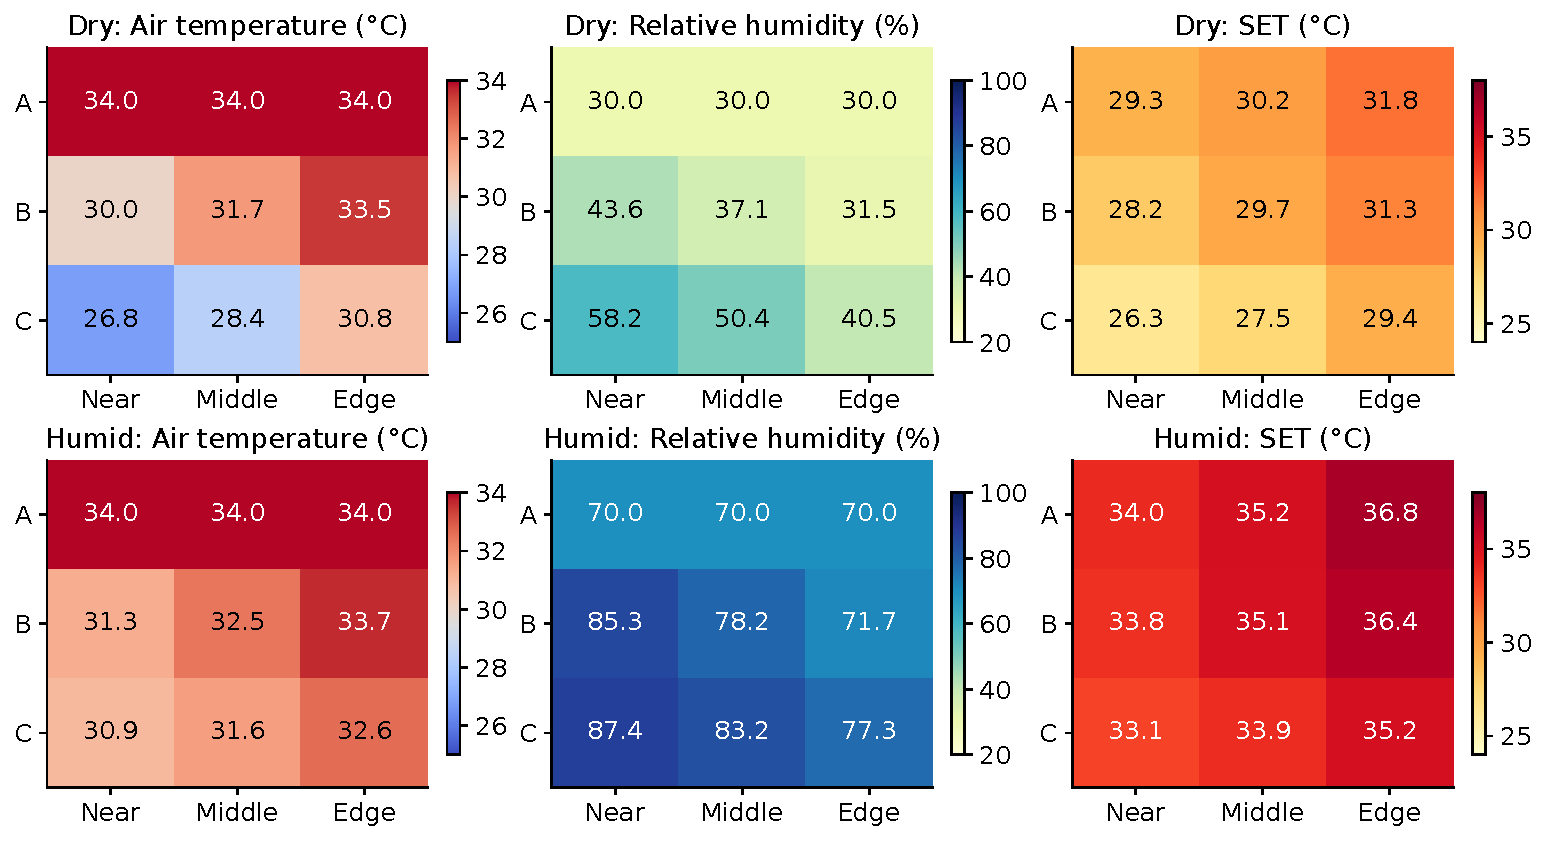
\includegraphics[width=0.88\linewidth]{figures/01_local_conditions.pdf}
\caption{Local conditions under the bus inputs: A changes SET through airflow; B/C also change temperature and moisture.}
\label{fig:bus-local}
\end{figure}
For C, dry-case SET rises from $26.3\,^{\circ}\mathrm C$ near the outlet to $29.4\,^{\circ}\mathrm C$ at the edge; at RH $70\%$, it rises from $33.1$ to $35.2\,^{\circ}\mathrm C$. These gradients explain why a single air-temperature drop misses delivered service.

\begin{figure}[!ht]
\centering
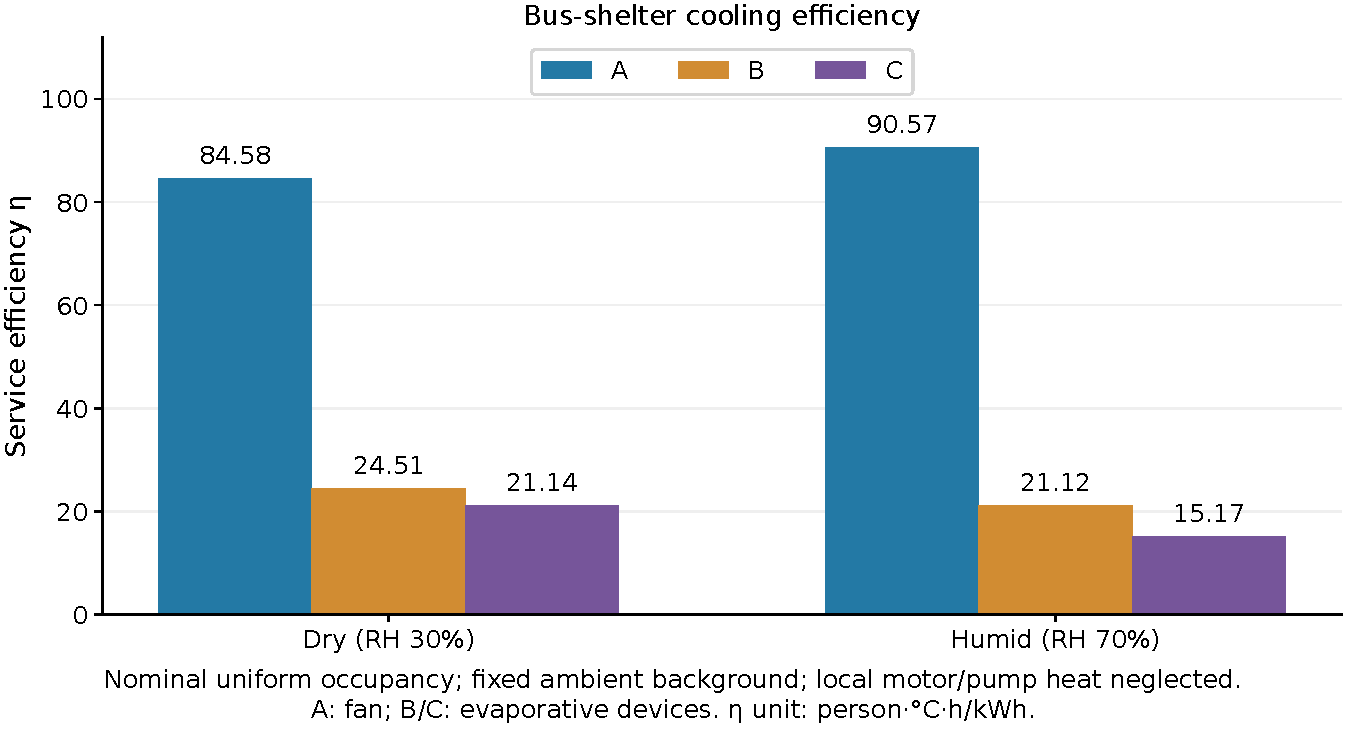
\includegraphics[width=0.76\linewidth]{figures/24_bus_efficiency.pdf}
\caption{Uniform-occupancy efficiency: A leads both nominal humidity cases.}
\label{fig:bus-efficiency}
\end{figure}
Dry-case efficiencies are $84.6/24.5/21.1$ for A/B/C; humid-case values are $90.6/21.1/15.2$ (Figure~\ref{fig:bus-efficiency}). B/C outlet drops fall from $5/8\,^{\circ}\mathrm C$ to about $3.4/3.4\,^{\circ}\mathrm C$, as their common wet-bulb limit replaces the caps.

\begin{figure}[!ht]
\centering
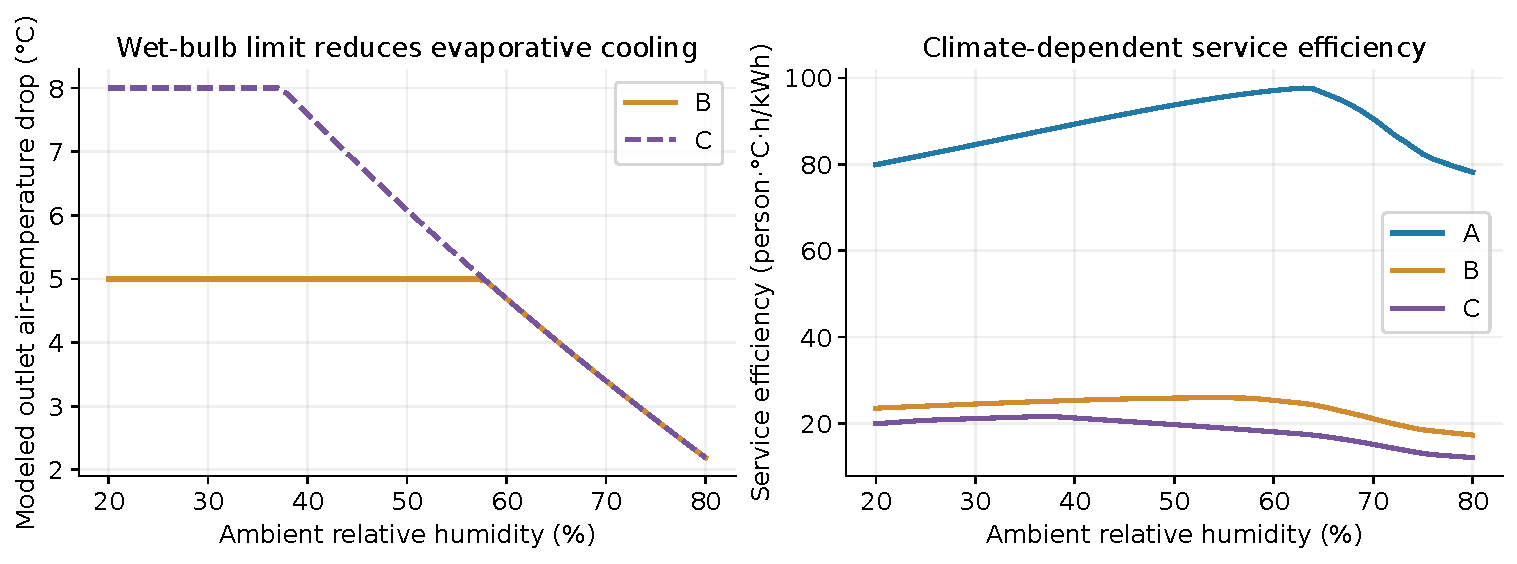
\includegraphics[width=0.88\linewidth]{figures/03_humidity_sweep.pdf}
\caption{Humidity changes evaporative potential and SET-based efficiency at fixed delivery and demand.}
\label{fig:bus-humidity}
\end{figure}
Moving the same 12 people toward the edge lowers dry-case A efficiency from $118.3$ to $48.3$ and reverses B/C ordering: $24.5>21.1$ under uniform occupancy becomes $15.5<16.6$ under edge-heavy occupancy. A leads all six nominal climate--occupancy cases.

\subsection{Delivery failure and robustness}
Aiming or obstruction can weaken delivered airflow without reducing power. Holding $p_A=0.25$ kW, test
\begin{equation}
 v_{A,z}(q)=v_0+q(v_{A,z}^{\mathrm{nom}}-v_0),\qquad 0\leq q\leq1,
\end{equation}
$q$ is a delivery factor, not a motor-speed setting. On the sampled grid, A first wins at $q=0.18$ for RH $30\%$ and $0.16$ for RH $70\%$; the threshold lies within the preceding $0.02$ interval. B wins below it.

\begin{figure}[!ht]
\centering
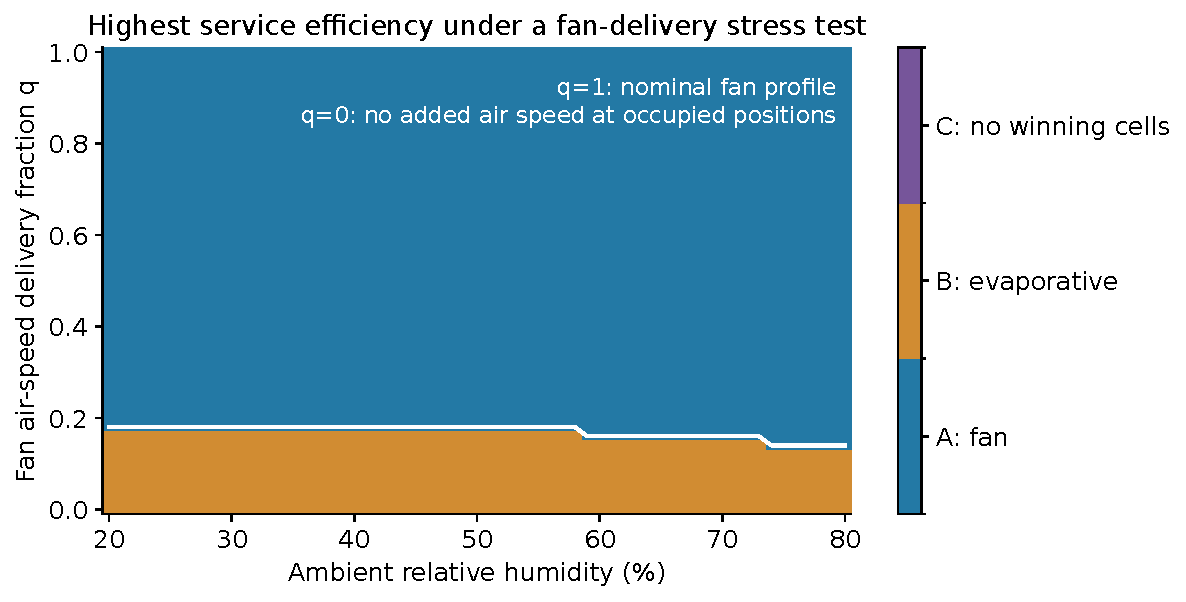
\includegraphics[width=0.79\linewidth]{figures/05_delivery_decision.pdf}
\caption{Efficiency winner for RH $20$--$80\%$ and delivered-speed factor $q$; C wins no cell of this grid.}
\label{fig:bus-decision}
\end{figure}
One-factor endpoint tests give maximum B/A and C/A efficiency ratios $0.432$ and $0.372$. Including full local electric heating ($\chi=1$) changes dry-case efficiencies to $81.0/20.8/18.0$ and humid values to $86.8/17.4/12.1$; A remains first under those inputs. Psychrometric round trips, mass/enthalpy closure, $U+R=R_0$, zero-occupancy and signed-adverse checks pass. The delivery-loss reversal identifies a stronger sensitivity than these individual endpoint perturbations.
\subsection{Extreme dry heat: testing the efficiency ranking}
We test $T_a=T_r=40\,^{\circ}\mathrm C$ at RH 15\% and 20\%, retaining the device powers, delivery profiles, 5/8$\,^{\circ}\mathrm C$ outlet caps, and uniform occupancy. Figure~\ref{fig:extreme-heat} shows $\eta_A>\eta_B>\eta_C$ in both cases. At RH 15\%, the mean SET reductions are 1.43, 1.95, and 3.42$\,^{\circ}\mathrm C$, whereas the efficiencies are 68.43, 19.48, and 16.41 person$\cdot{}^{\circ}\mathrm C\cdot$h/kWh. C produces greater relief per passenger, but consumes ten times A's electricity. SET relief explains the service numerator; $\eta$ remains the comparison criterion.

The heat balance explains why dry-bulb cooling alone cannot establish the ranking. When air is warmer than the exposed skin or clothing surface, faster flow increases convective heat gain; it also promotes evaporative heat loss. SET combines these competing exchanges rather than imposing a temperature-triggered reversal of fan performance \cite{thermalcomfort}.

\begin{figure}[htbp]
\centering
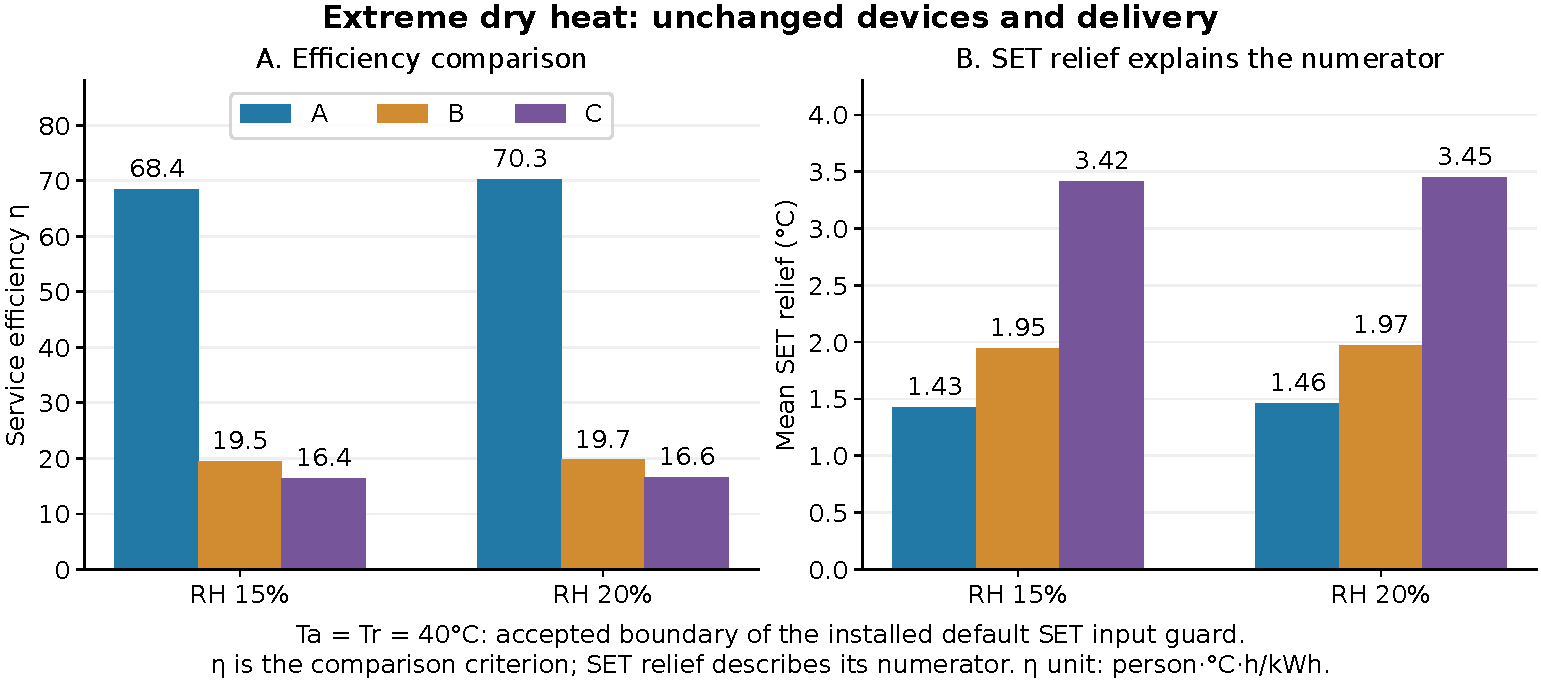
\includegraphics[width=.85\textwidth]{figures/26_extreme_heat.pdf}
\caption{Extreme dry-heat boundary test with the original device powers and delivery profiles. The left panel compares cooling efficiency; the right panel explains its SET-relief numerator. Inputs follow Assumption A4.}
\label{fig:extreme-heat}
\end{figure}


\section[Rail station]{Canberra Station: Dynamic Background and Local Service}
\label{sec:rail}

\subsection{From a fixed reservoir to coupled zones}
Canberra MRT is an elevated, naturally ventilated station in Singapore \cite{canberra-rsp,canberra-lta}. Using its approximate $L=220$ m length with assumed aggregate waiting width $b=6$ m and usable fraction $\alpha=0.8$ gives
\begin{equation}
 A_{\mathrm{occ}}=\alpha Lb=1056\,\mathrm{m^2}.
\label{eq:canberra-area}
\end{equation}
Three access/core/edge zones each have $352\,\mathrm{m^2}$ and, at 4 m effective height, $1408\,\mathrm{m^3}$. Table~\ref{tab:rail-inputs} defines the $33\,^{\circ}\mathrm C$, RH $70\%$ comparison. Its $4$--$10$ h$^{-1}$ background exchange implies 6--15 min replacement times, comparable to the 15-min passenger cycle: storage and humidity feedback must now be resolved.

\begin{figure}[!ht]
\centering
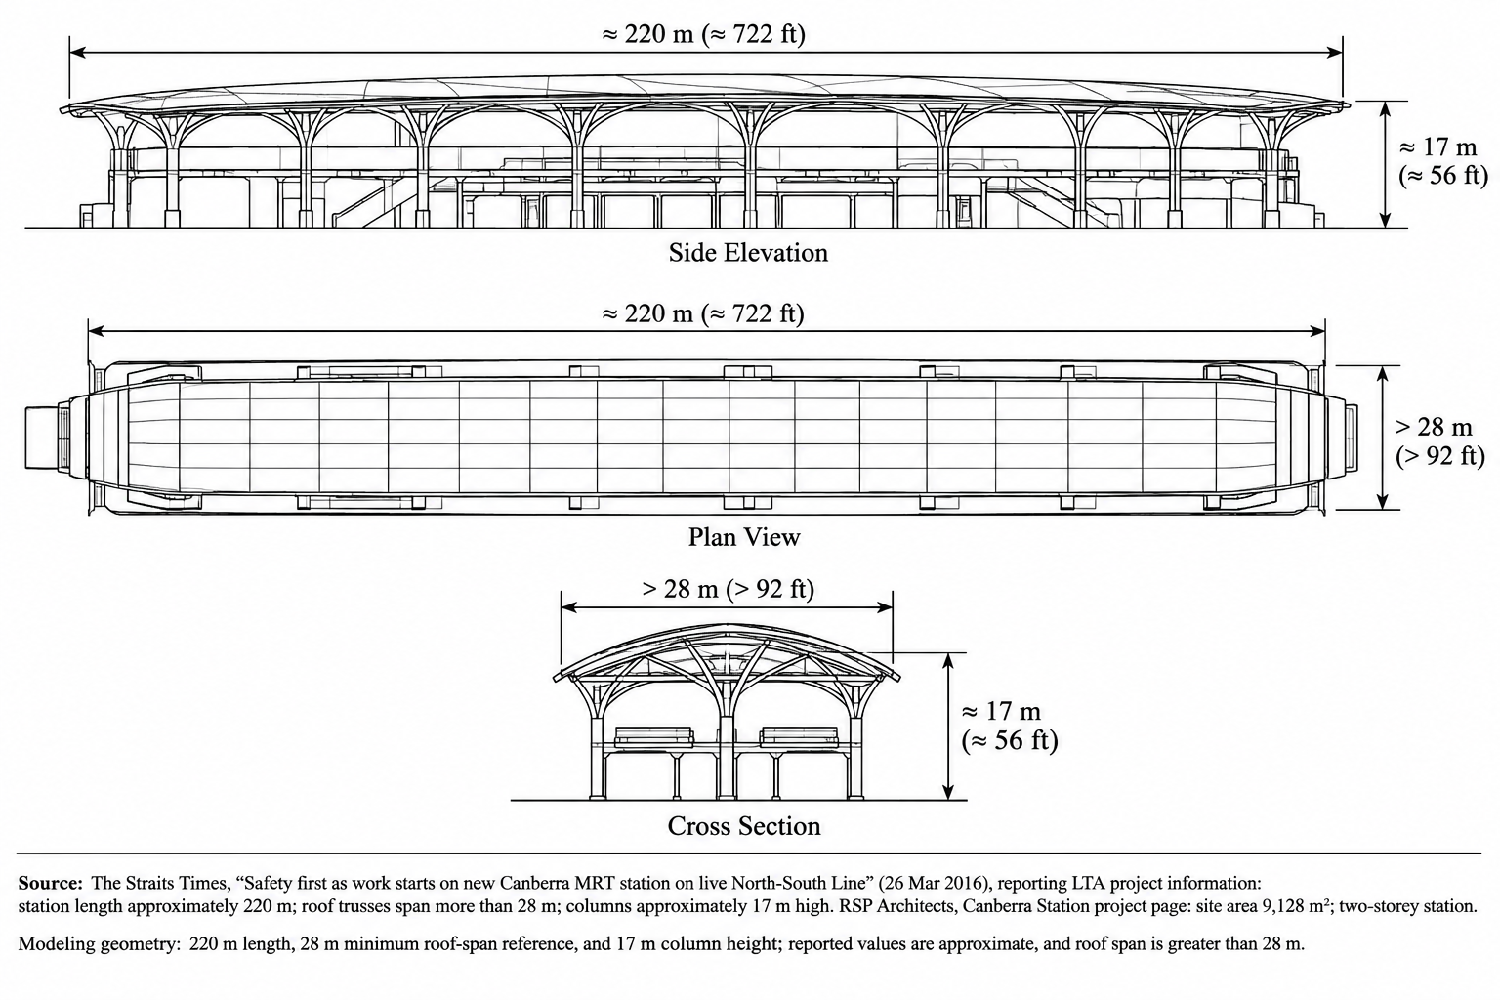
\includegraphics[width=0.66\linewidth]{figures/13_canberra_station.pdf}
\caption{Canberra station context. Structural dimensions guide scale; the three waiting zones are modeled separately \cite{canberra-dimensions,canberra-rsp}.}
\label{fig:canberra}
\end{figure}

Each zone retains $h_z,w_z$ and effective surface temperature $T_{m,z}$, with constant reference dry-air mass $M_z=\rho_{da,o}V_z$. The device, local-mixing and SET operators remain those of the bus. For $x=h$ or $w$, balanced exchange is
\begin{equation}
 \mathcal L_z(x)=\dot m_{0z}(x_o-x_z)+\sum_{j\ne z}\dot m_{zj}(x_j-x_z),
 \qquad \dot m_{0z}=M_z\lambda_z/3600.
\label{eq:rail-exchange}
\end{equation}
$\lambda_z$ is ACH in h$^{-1}$; interzone rates satisfy $\dot m_{zj}=\dot m_{jz}$. Outdoor exchange represents wind/opening effects through the prescribed cycle \cite{ventilation}. With time in seconds, the three conservation equations per zone are \cite{epzone}
\begin{align}
 M_z\dot h_z={}&\mathcal L_z(h)+H_{ma,z}(T_{m,z}-T_z)
 +n_zq_c+n_zg h_v(T_z)+P_z
 +\sum_k x_{zk}\dot m_k(h_{e,zk}-h_z),\label{eq:rail-enthalpy}\\
 M_z\dot w_z={}&\mathcal L_z(w)+n_zg+
 \sum_k x_{zk}\dot m_k(w_{e,zk}-w_z),\label{eq:rail-moisture}\\
 C_{m,z}\dot T_{m,z}={}&H_{mo,z}(T_o-T_{m,z})+Q_{\mathrm{sol},z}
 +n_zq_r-H_{ma,z}(T_{m,z}-T_z).\label{eq:rail-surface}
\end{align}
Here $n_z$ is occupancy; per-person $q_c,q_r$ are convective/radiant W and $g$ is vapor kg/s. Vapor enthalpy is $h_v(T)=2501000+1860T$ J/kg, with no second latent term. $H_{ma},H_{mo}$ are W/K, $C_m$ is J/K, $Q_{\rm sol}$ is W, and $P_z=\sum_kx_{zk}P_k$ with $P_k=1000p_k$ W. Subscript $e$ denotes the unheated device outlet (the bus's $o,s$), so A has no evaporative source; B/C add moisture while approximately conserving outlet enthalpy. Surface exchange cancels between the air and wall budgets.

Recover $T_z=(h_z-2501000w_z)/(1006+1860w_z)$; effective view fraction $F_z$ determines mean radiant temperature \cite{thermalcomfort}:
\begin{equation}
 T_{r,z}=\left[F_z(T_{m,z}+273.15)^4+(1-F_z)(T_{r,o}+273.15)^4\right]^{1/4}-273.15.
\label{eq:rail-mrt}
\end{equation}
The separate outdoor radiant input is $T_{r,o}$. Increasing $w_z$ reduces the next device pass's wet-bulb depression, providing the feedback absent from the fixed-background bus.

\subsection{Local delivery with exact return accounting}
Device flow and entrained background return to their original zone. For finite entrainment ($\beta>0$), the local mixing equations imply
\begin{align}
 (\dot m_k+\dot m_e)(h_{\ell,zk}-h_z)+(1-\chi)P_k
 &=\dot m_k(h_{e,zk}-h_z)+P_k,\\
 (\dot m_k+\dot m_e)(w_{\ell,zk}-w_z)
 &=\dot m_k(w_{e,zk}-w_z).
\label{eq:return-closure}
\end{align}
Thus the local exposure calculation preserves the existing net heat and moisture sources exactly. Covered people use local $T,\phi,v$; uncovered people use background $T,\phi,v_0$, and both share $T_r$. Here $\beta=0.5$, $\chi=1$ and A/B/C unit flows are $0.6/0.6/1.2$ kg dry air/s under Table~\ref{tab:rail-inputs}; $\chi=1$ places all electrical heat in supply before passengers.

Two reductions identify the inheritance precisely. At $\beta=0$, the scalar exposure becomes the original shared-background calculation while prescribed speeds remain. Fixing background to outdoor $h_a,w_a$, using bus radiation, speeds, occupancy and $\beta$, and setting $\chi=0$ recovers the bus calculation exactly. Setting time derivatives to zero alone would not impose that reservoir boundary.

\subsection{Counts, coverage and efficiency}
Let $s$ index an installation and $x_{zk}$ its nonnegative integer count of type $k$ in zone $z$. For unit footprints $a_{A/B/C}=20/30/40\,\mathrm{m^2}$, uniform zone density gives
\begin{equation}
 c_{zk}=\frac{x_{zk}a_k}{A_z},\qquad
 c_{z0}=1-\sum_k c_{zk}\ge0,\qquad \sum_kx_{zk}a_k\le A_z.
\label{eq:coverage}
\end{equation}
These passenger fractions $c$ differ from the air-mixing fraction $\beta$. Average discomfort across subgroups, not velocities or device efficiencies:
\begin{equation}
 \overline D_{s,z}(t)=c_{z0}D[\Theta(T_z,T_{r,z},v_0,\phi_z)]
 +\sum_k c_{zk}D[\Theta(T_{\ell,zk},T_{r,z},v_{zk},\phi_{\ell,zk})].
\label{eq:mixed-discomfort}
\end{equation}
All units affect the background; direct coverage determines the additional local exposure. Every plan starts after the same two-hour uncooled warm-up, runs two hours, and uses a matched no-device baseline. The common passenger history totals 440 person-hours. With $p_k$ in kW,
\begin{align}
 U_s&=\frac1{3600}\int_0^{7200}\sum_z n_z(t)[D_{0,z}(t)-\overline D_{s,z}(t)]\,dt,\\
 E_s&=\frac1{3600}\int_0^{7200}\sum_{z,k}x_{zk}p_k\,dt,
 \qquad \eta_s=U_s/E_s.
\label{eq:rail-efficiency}
\end{align}
The $1/3600$ factors convert seconds to hours, retaining person$\cdot{}^{\circ}\mathrm C\cdot$h/kWh. This section compares $U/E$. Mean residual $\overline R_s=\int\sum_z n_z\overline D_{s,z}\,dt/\int\sum_z n_z\,dt$ supplies the later adequacy criterion in Section~\ref{sec:effectiveness}.

\subsection{Deployment results and verification}
Among 24 sampled plans, A3 maximizes $\eta$ at $37.58$; among the six equal-$68.18\%$-coverage benchmarks, A36 leads at $35.49$. The distinct candidate sets answer scale and device-comparison questions, respectively (Figure~\ref{fig:deployment-efficiency}).

Plan suffixes give total device counts. For A36/B24/C18/AB30/AC27/ABC24, per-zone $(A,B,C)$ counts are $(12,0,0)$, $(0,8,0)$, $(0,0,6)$, $(6,4,0)$, $(6,0,3)$ and $(3,2,3)$, respectively; A3 places one fan in each zone.

\begin{table}[!ht]
\centering\small
\caption{Nominal efficiency accounting: $U$ in person$\cdot{}^{\circ}$C$\cdot$h, $E$ in kWh.}
\label{tab:deployment-results}
\begin{tabular}{@{}lrrrr@{}}
\toprule
Plan & Person-time coverage & $U$ & $E$ & $\eta$\\
\midrule
A3 & 5.68\% & 56.38 & 1.5 & 37.58\\
A36 & 68.18\% & 638.89 & 18.0 & 35.49\\
B24 & 68.18\% & 446.28 & 57.6 & 7.75\\
C18 & 68.18\% & 453.00 & 90.0 & 5.03\\
AB30 & 68.18\% & 581.61 & 37.8 & 15.39\\
AC27 & 68.18\% & 593.68 & 54.0 & 10.99\\
ABC24 & 68.18\% & 524.76 & 63.9 & 8.21\\
AB30-R & 76.19\% & 695.07 & 37.8 & 18.39\\
\bottomrule
\end{tabular}
\end{table}

Redistributing AB30's 18 A and 12 B units to zone counts $(3,4,0)$, $(12,3,0)$ and $(3,5,0)$ raises person-time coverage from $68.18\%$ to $76.19\%$. At the same 37.8 kWh, $U$ rises from $581.61$ to $695.07$ and $\eta$ from $15.39$ to $18.39$: allocation changes useful delivery without adding equipment.

A36 retains its equal-coverage efficiency lead for all 15 combinations $\beta=0/0.25/0.5/0.75/1$, $\chi=0/0.5/1$. Varying A's unit flow through $0.3/0.6/1.2$ kg dry air/s gives efficiencies $34.06/35.49/36.22$. Figure~\ref{fig:local-sensitivity} shows the controlled delivery sensitivity.


\begin{figure}[!ht]
\centering
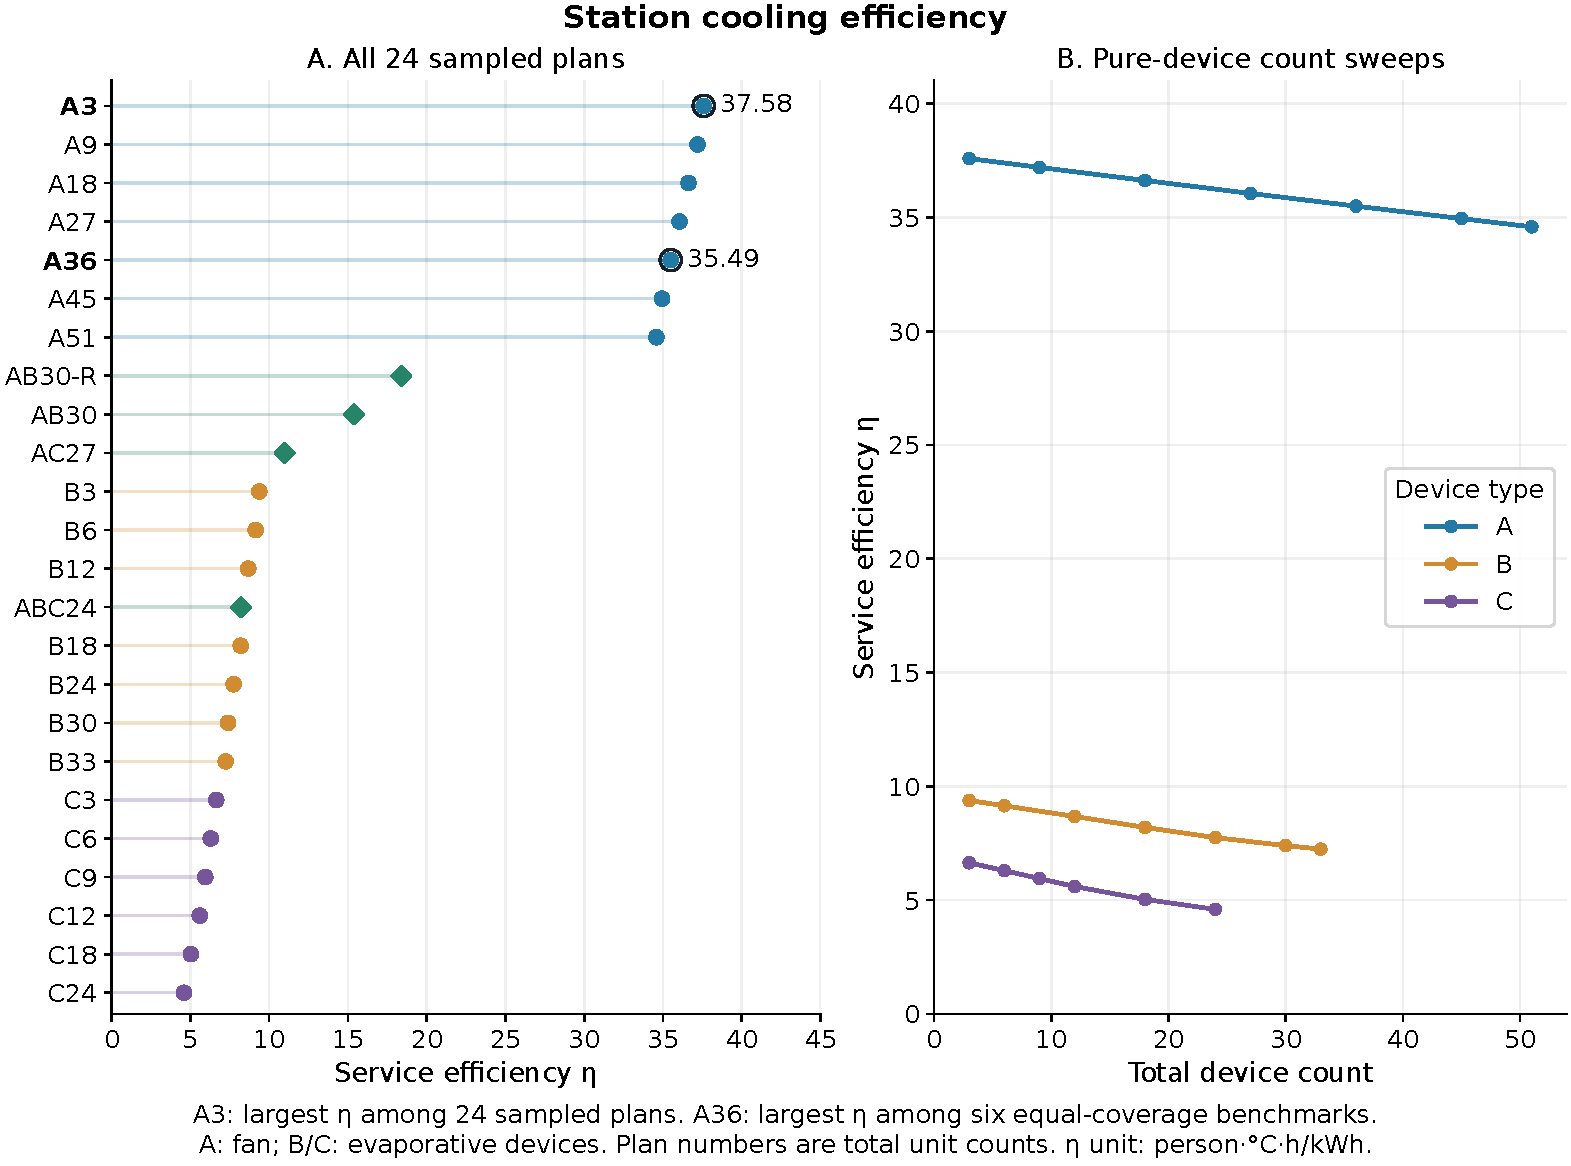
\includegraphics[width=0.88\linewidth]{figures/22_station_efficiency.pdf}
\caption{A3 leads all 24 sampled installations; A36 leads the six equal-coverage benchmarks. Device counts change both delivered service and background loads.}
\label{fig:deployment-efficiency}
\end{figure}

\begin{figure}[!ht]
\centering
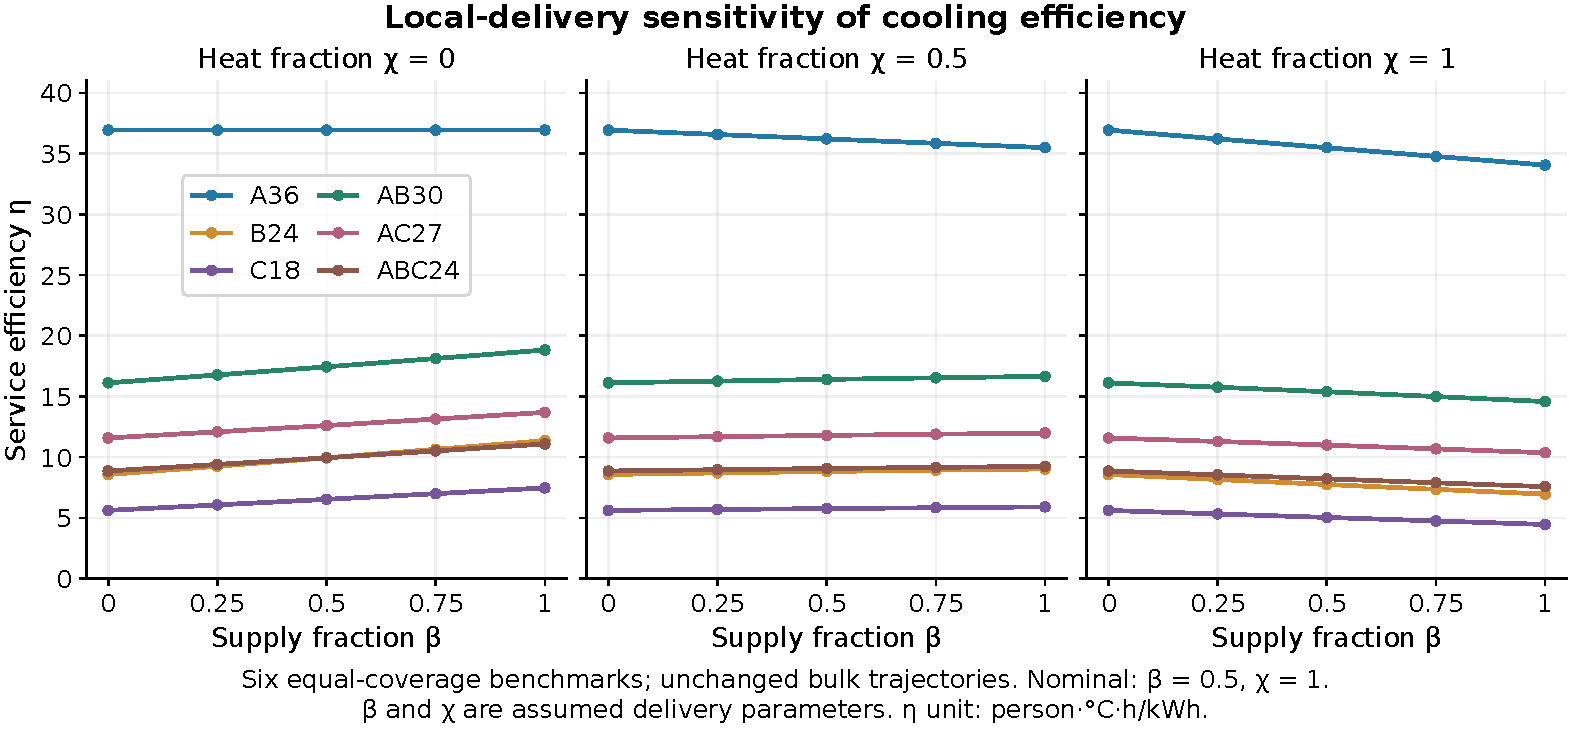
\includegraphics[width=0.88\linewidth]{figures/23_delivery_efficiency.pdf}
\caption{Efficiency sensitivity to mixing and heat allocation; background trajectories remain unchanged by the local mapping.}
\label{fig:local-sensitivity}
\end{figure}

Global energy/moisture budgets and local return identities close numerically. Halving the time step changes the tested mixed-plan efficiencies by at most $5.4\times10^{-6}$ relatively; $\beta=0$ reproduces all 24 former shared-background results exactly. The fixed-reservoir test recovers bus states and service. These checks verify the extension's conservation and reduction properties.
\FloatBarrier
\IfFileExists{sections/applications.tex}{\section[Venue applications]{Apply the Model: Two Outdoor Dining Venues}
\label{sec:applications}

\subsection{Different climates, the same service calculation}
We apply CP-SET to a dining sector of \textbf{Ullman Terrace at Desert Botanical Garden, Phoenix}, an outdoor event patio \cite{ullman}, and \textbf{Satay Street at Lau Pa Sat, Singapore}, an open-air dining street on Boon Tat Street \cite{satay-street}. Their dry-desert and humid-tropical climate contrast is represented by the warm-day scenarios in Table~\ref{tab:venue-inputs}.

Both spaces are open enough for a prescribed-background planning approximation. We retain the bus model's device outlets, enthalpy--moisture mixing, local-speed profiles and SET calculation, together with the station model's integer allocation and disjoint coverage. Three delivery strips within each device footprint represent attenuation from its near to far edge. Their equal-weight mean excess is $D_k=\frac13\sum_{j=1}^{3}D(\Theta_{kj})$. With the coverage fractions $c_{zk}$ from Eq.~\eqref{eq:coverage},
\begin{equation}
 \overline R_s=\frac{\sum_z n_z\left[(1-\sum_k c_{zk})D_0+
                  \sum_k c_{zk}D_k\right]}{\sum_z n_z},\qquad
 U_s=H\Big(\sum_z n_z\Big)(D_0-\overline R_s).
\label{eq:venue-service}
\end{equation}
Thus geometry controls who receives relief, while $E_s=H\sum_{z,k}x_{zk}p_k$ counts every device. The supply flow used for water demand belongs to each physical device, not separately to each delivery strip. Fixed background and $\chi=0$ retain the shelter approximation; crowd-driven accumulation or poorly flushed enclosures require the dynamic station equations instead.

\subsection{Climate changes the value of evaporation}
Task 3 ranks $\eta$ over every positive-energy layout satisfying nonoverlap: $12{,}166$ in Phoenix and $3{,}374$ in Singapore. \textbf{The maximum efficiencies are $81.10$ and $134.89$ person$\cdot{}^\circ$C$\cdot$h/kWh.} A single fan in the busiest zone attains each maximum, covering $10\%$ and $12.5\%$ of guest-time, respectively. Up to five such fans in Phoenix and four in Singapore tie while remaining inside that zone; no coverage, cost or residual threshold enters this efficiency ranking.

Table~\ref{tab:venue-results} separately compares pure types at the same coverage. Within each type, we choose the least-energy layout achieving that coverage. The wet-bulb temperatures are $20.90^\circ$C in Phoenix and $28.16^\circ$C in Singapore. Consequently, C achieves its $8^\circ$C outlet-drop cap in the dry scenario, but only $2.68^\circ$C in the humid scenario. Dilution and the SET response translate this outlet change into useful service.

\begin{table}[!ht]
\centering\small
\caption{Equal-coverage efficiency comparison: every plan serves $60\%$ of guest-time. $U$ is person$\cdot{}^\circ$C$\cdot$h and $\eta=U/E$.}
\label{tab:venue-results}
\begin{tabular}{@{}llrrr@{}}
\toprule
Venue & Plan & $U$ & $E$ (kWh) & $\eta$\\
\midrule
Phoenix & A7 & 486.58 & 7.0 & 69.51\\
 & B5 & 666.41 & 24.0 & 27.77\\
 & C4 & 1183.98 & 40.0 & 29.60\\
Singapore & A6 & 647.48 & 6.0 & 107.91\\
 & B4 & 728.44 & 19.2 & 37.94\\
 & C3 & 1069.98 & 30.0 & 35.67\\
\bottomrule
\end{tabular}
\end{table}

Fans give the greatest service per kWh in both comparisons. The B--C efficiency order reverses: C exceeds B in Phoenix, whereas B exceeds C in Singapore. Humidity removes C's larger outlet-temperature-drop advantage, leaving delivery reach and unit power to determine its efficiency. Singapore's larger fan efficiency also reflects its denser dining sector and stronger modeled SET response to air movement. Occupancy, delivery and climate therefore belong in the same calculation.

\begin{figure}[!ht]
\centering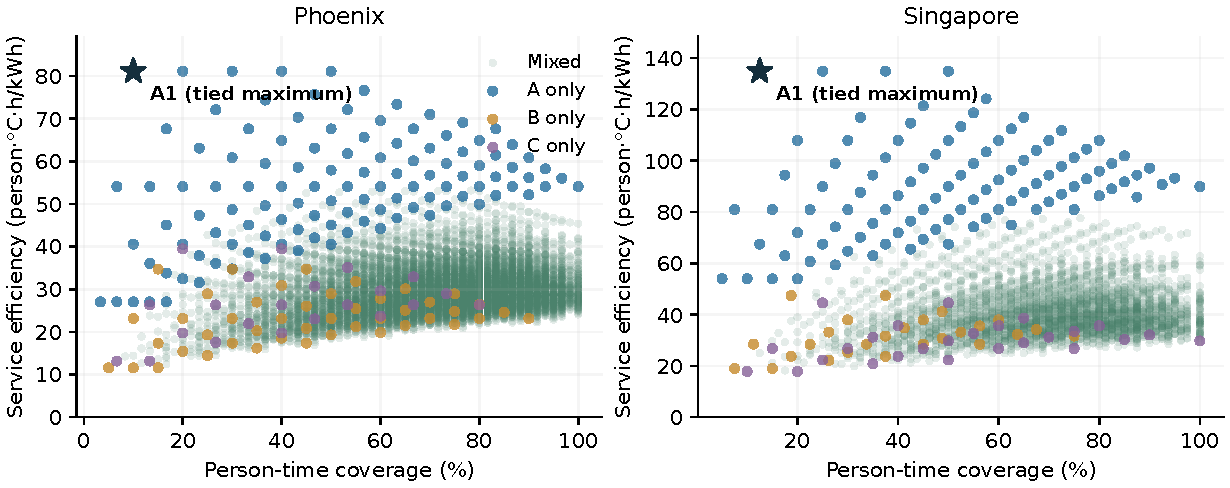
\includegraphics[width=\linewidth]{figures/27_venue_comparison.pdf}
\caption{Efficiency over all positive-energy integer layouts, with no coverage threshold. Coincident points are merged for display. Stars identify the smallest installations attaining the tied maximum; broader service changes the relevant occupied locations.}
\label{fig:venue-comparison}
\end{figure}

\subsection{What scales, and what does not}
Efficient cooling depends chiefly on delivering air to occupied locations, preserving useful speed, limiting dilution, and exploiting a sufficient dry-bulb--wet-bulb difference. Increasing area changes the equipment count and occupied-location weights; it does not multiply $\eta$ directly.

A scale check makes this distinction concrete. Doubling Singapore's area and guests at the same density, while retaining the reference fan layout $(4,4,2)$, leaves $U/E=97.12$ unchanged but halves coverage from $90\%$ to $45\%$. Doubling the devices as well restores coverage, doubles electricity from $10$ to $20$ kWh, and again preserves $U/E$. Efficiency is therefore an intensity measure; service adequacy enters the next task. The code verifies these scaling identities, $U+R=R_0$, saturation bounds and the shared heat/moisture conservation checks.

}{}
\IfFileExists{sections/effectiveness_complete.tex}{\section[Cooling effectiveness]{Overall Effectiveness: Four Objectives, an Explicit Choice}
\label{sec:effectiveness}

\subsection{Performance, access, energy and cost}
We retain the physical outputs and compare four quantities,
\begin{equation}
 \min_s\big(\overline R_s,\ X_s,\ E_{s,y},\ C_{s,y}\big),\qquad
 X_s=\frac{\sum_{z,k}x_{zk}b_k}{\sum_z A_z}.
\label{eq:effectiveness-vector}
\end{equation}
Remaining SET excess measures thermal performance. $X_s$ is the fraction of dining area reserved for equipment and maintenance clearance, providing a calculable \textit{visitor-access proxy}. Clear walkways and exits remain layout requirements. $E_{s,y}$ measures resource use, and $C_{s,y}$ measures annual expenditure. Thermal relief is counted once; $\eta$ is not a fifth objective.

All ownership, maintenance and running costs use the annual basis in Table~\ref{tab:venue-inputs}. With capital recovery factor $\operatorname{CRF}=r(1+r)^L/[(1+r)^L-1]$,
\begin{equation}
 \begin{aligned}
 C_{s,y}&=\operatorname{CRF}\sum_{z,k}x_{zk}K_k+
             \sum_{z,k}x_{zk}M_k+\pi_eE_{s,y}+\pi_wV_{s,y},\\
 V_{s,y}&=\frac{3600H_y\lambda_w}{\rho_w}
          \sum_{z,k}x_{zk}\dot m_k(w_{e,k}-w_a).
 \end{aligned}
\label{eq:venue-cost}
\end{equation}
Here $K_k$ and $M_k$ are initial and annual maintenance costs, $H_y$ is annual operating hours, and $\rho_w$ converts evaporated mass to water volume. The common USD price basis supports comparison. EIA's Arizona commercial average, USD $0.1245$/kWh in 2025 \cite{eia-commercial}, falls within the electricity sensitivity range.

\subsection{Conditional recommendations from the full candidate set}
For Task 4, we impose the assumed coverage requirement, then remove four-objective dominated options. Phoenix/Singapore have $199/106$ eligible count combinations and $80/32$ \textbf{coverage-constrained Pareto options}. For identical counts, energy, cost and clearance are position-independent here; retaining the eligible layout with least residual therefore preserves the policy optimum. Under an illustrative operator policy,
\begin{equation}
 s^*=\arg\min_s C_{s,y}\quad\text{subject to}\quad
 q_s\ge q_{\min},\quad\overline R_s\le\overline R_{\max},\quad
 X_s\le X_{\max},\quad E_{s,y}\le E_{\max}.
\label{eq:effectiveness-selection}
\end{equation}
The limits in Table~\ref{tab:venue-inputs} express a budgeted service choice without arbitrary equal weighting. Exhaustive enumeration establishes the minimum within the discrete design space.

\begin{table}[!ht]
\centering\small
\caption{Selected plans under the stated four-objective policy. Annual costs include ownership, maintenance, electricity and water.}
\label{tab:venue-decisions}
\begin{tabular}{@{}llrrrrr@{}}
\toprule
Venue & Plan & $q$ (\%) & $\overline R$ ($^\circ$C) & $X$ (\%) & $E_y$ (kWh) & $C_y$ (USD)\\
\midrule
Phoenix & A10C2 & 96.67 & 4.482 & 2.67 & 4500 & 3360\\
Singapore & A10 & 90.00 & 7.453 & 2.08 & 1500 & 1293\\
\bottomrule
\end{tabular}
\end{table}

In Phoenix, place two C units and one A in the busiest zone, five A units in the second, and four A in the third. This A10C2 layout delivers $1248.87$ person$\cdot{}^\circ$C$\cdot$h per session using $30$ kWh and $0.319$ m$^3$ of make-up water. A15 is cheaper but misses the residual requirement; C6 exceeds the energy budget. In Singapore, the A allocation $(4,4,2)$ meets the policy with $971.22$ service units and $10$ kWh. Its ten fans require no evaporative make-up water. The different choices emerge from the constraints and climate response.

\begin{figure}[!ht]
\centering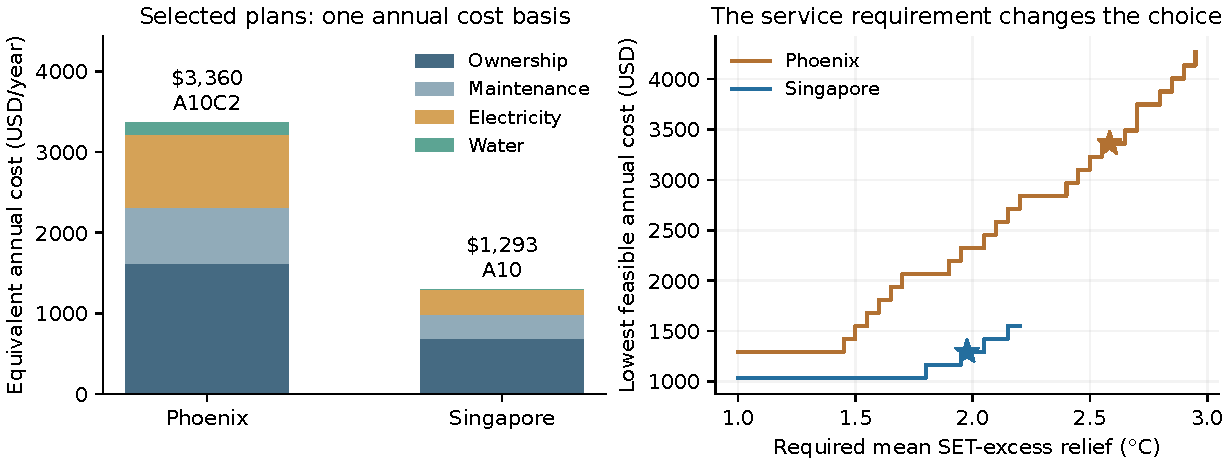
\includegraphics[width=\linewidth]{figures/28_effectiveness.pdf}
\caption{Annual costs of the selected plans and the minimum cost as the required thermal relief increases, holding the other policy limits fixed. Stars mark the stated policy. Stepped curves reflect integer equipment choices.}
\label{fig:venue-effectiveness}
\end{figure}

\subsection{Sensitivity leads to an operating policy}
Across $243$ price combinations, Phoenix retains A10C2 in $228$ ($93.8\%$) and selects A4C3 in $15$; Singapore retains A10 throughout. Physical changes have stronger effects in these tests. A $0.15$ loss in evaporative delivery fraction selects A6C3 in Phoenix; a $20\%$ loss in induced speed selects A7C3 there and A12 in Singapore. Raising RH by ten percentage points leaves both venues without a feasible layout under their unchanged service, access and energy policies. Operators should then revise timing, radiant exposure or the service budget and reoptimize. The memorandum translates these triggers into operating actions.
}{}
\IfFileExists{sections/operator_memo.tex}{\clearpage
\section*{Memorandum to the Chief Operations Officer}
\addcontentsline{toc}{section}{Memorandum to the COO}
\noindent\textbf{To:} Chief Operations Officer, HiMCM\\
\textbf{From:} Cooling-service modeling team\\
\textbf{Subject:} A targeted cooling plan for the modeled warm-day dining event

We recommend that HiMCM use \textbf{ten type-A fans and two type-C evaporative units} as the planning configuration for the modeled $300$-m$^2$, $120$-guest sector at Ullman Terrace. The venue's operations team can implement the layout under the $36^\circ$C, $25\%$ RH design condition and the service, access and annual-energy limits in our analysis.

Put both evaporative units and one fan in the busiest zone, five fans in the next, and four in the least crowded zone. This arrangement directs the strongest cooling to the greatest number of guests. The model estimates $96.7\%$ person-time coverage and an average reduction of $2.60^\circ$C in SET excess. A four-hour event uses \textbf{30 kWh and approximately 319 liters of make-up water}. Its service efficiency is $41.63$ person$\cdot{}^\circ$C$\cdot$h/kWh. Remaining SET excess is $4.48^\circ$C, so substantial warmth remains despite the improvement.

Under our common price assumptions, initial equipment expenditure is \textbf{USD 7,000}; equivalent annual cost is approximately \textbf{USD 3,360} at 600 operating hours. This annual figure includes capital recovery, maintenance, electricity and water. Obtain installation and operating quotes before purchase. Fifteen fans alone cost less but miss our specified thermal-relief target. Six C units provide stronger relief but exceed the chosen annual electricity budget.

The installation needs a commissioning check. Confirm that the assumed delivery footprints and air speeds reach seated guests, while equipment, hoses and servicing space leave circulation routes and exits clear. Record conditions near, midway from and at the edge of each representative unit. Recalculate the plan when readings differ from the assumed profiles. If induced air speed is $20\%$ lower, the model selects seven fans and three C units under the same policy. A less effective evaporative delivery profile instead selects six fans and three C units; each trigger is evaluated separately.

Humidity is an important operating trigger. At $35\%$ RH with other Phoenix inputs unchanged, no enumerated layout meets the original thermal target under the unchanged service, access and energy policy. Review timing, shade and the approved service requirement before adding equipment. Follow National Weather Service heat guidance: monitor forecasts, reduce or reschedule strenuous outdoor activity, and provide breaks and access to cooler locations \cite{nws-heat}.

}{}
\IfFileExists{sections/public_blog.tex}{\clearpage
\section*{Public Blog: How Much Comfort Does One Kilowatt-Hour Buy?}
\addcontentsline{toc}{section}{Public blog}

An outdoor fan can help people feel cooler while the air thermometer barely changes. An evaporative cooler can lower air temperature while adding moisture. To compare them fairly, we followed the cooling all the way to the guest: what temperature, humidity, air movement and radiant heat reach that person, and how long do they benefit?

Our model uses Standard Effective Temperature, or SET, to combine those influences into one thermal-response measure. We track relief above a stated reference condition, then divide the total person-time benefit by electricity use. One service unit means one person's SET excess is reduced by one degree for one hour. This is a model-based comfort measure, not a degree of outdoor air cooling or a unit of heat extracted.

Consider our Singapore dining scenario: 120 guests, four hours, and ten carefully placed fans. The calculation gives about \textbf{971 service units for 10 kWh}, or \textbf{97 service units per kWh}. Across all guests, that corresponds to roughly two degrees less SET excess during the event. The fans directly serve about 90\% of guest-time.

The Phoenix example needs a different choice to meet its service target. Ten fans plus two evaporative units supply about \textbf{1,249 service units for 30 kWh}: about \textbf{42 per kWh}. Dry air leaves more room for water to evaporate, but equipment power, delivery losses and where people sit still matter. A higher-powered cooler is worthwhile when its extra relief is needed and reaches enough guests.

One number cannot tell the whole story. Doubling the Singapore dining area and crowd while keeping ten fans leaves the efficiency ratio unchanged, yet halves coverage to 45\%. Check who is served, how much warmth remains, and what the equipment costs. During severe heat, follow local advisories and adjust outdoor plans \cite{nws-heat,nea-heat}.

}{}
\clearpage
\phantomsection\addcontentsline{toc}{section}{References}
\begin{thebibliography}{99}
\fontsize{9.5}{11}\selectfont
\urlstyle{same}
\setlength{\itemsep}{0pt}
\setlength{\parskip}{0pt}
\bibitem{ashrae}
ASHRAE. \emph{2026 ASHRAE Handbook---Refrigeration},
Chapter 15, \emph{Retail Food Store Refrigeration and Equipment}.
Product Temperatures and Display Refrigerator Cooling Load sections.
\url{https://handbook.ashrae.org/Handbooks/R26/IP/r26_ch15/r26_ch15_ip.aspx}.


\bibitem{etl}
UK Department for Energy Security and Net Zero.
\emph{Energy Technology List: Retrofit Measures for Open Fronted Refrigerated Display Cabinets}.
Definitions and product-temperature performance requirements.
\url{https://etl.energysecurity.gov.uk/products/refrigeration-equipment/retrofit-measures-open-fronted-refrigerated-display-cabinets}.


\bibitem{evap}
ASHRAE. \emph{2023 ASHRAE Handbook---HVAC Applications},
Chapter 53, \emph{Evaporative Cooling}.
\url{https://handbook.ashrae.org/Handbooks/A23/SI/A23_Ch53/a23_ch53_si.aspx}.


\bibitem{problem}
COMAP. \emph{2026 HiMCM Problem B: Air Conditioning the Environment: Modeling Energy Waste in Public Cooling}.
Requirements 1--5.

\bibitem{evapequip}
ASHRAE. \emph{2020 ASHRAE Handbook---HVAC Systems and Equipment},
Chapter 41, \emph{Evaporative Air-Cooling Equipment}, Section 1.
\url{https://handbook.ashrae.org/handbooks/S20/SI/s20_ch41/s20_ch41_si.aspx}.


\bibitem{fanguide}
Center for the Built Environment, University of California, Berkeley.
\emph{Fans for Cooling People Guidebook: Elevated Air Speed and Thermal Comfort}.
\url{https://cbe-berkeley.gitbook.io/fans-guidebook/full-guidebook/elevated-air-speed-and-thermal-comfort}.


\bibitem{thermalcomfort}
ASHRAE. \emph{2017 ASHRAE Handbook---Fundamentals},
Chapter 9, \emph{Thermal Comfort}, Section 10, Environmental Indices.
\url{https://handbook.ashrae.org/Handbooks/f17/IP/f17_ch09/f17_ch09_ip.aspx}.


\bibitem{pythermal}
Tartarini, F., and Schiavon, S. (2020).
pythermalcomfort: A Python package for thermal comfort research.
\emph{SoftwareX}, 12, 100578.
\url{https://doi.org/10.1016/j.softx.2020.100578}.
SET API and applicability limits:
\url{https://pythermalcomfort.readthedocs.io/en/stable/documentation/models.html}.


\bibitem{psychrolib}
Meyer, D., and Thevenard, D. (2019).
PsychroLib: a library of psychrometric functions to calculate thermodynamic properties of air.
\emph{Journal of Open Source Software}, 4(33), 1137.
\url{https://doi.org/10.21105/joss.01137}.
SI psychrometric API:
\url{https://psychrometrics.github.io/psychrolib/api_docs.html}.


\bibitem{nycshelter}
New York City Department of Transportation.
\emph{Street Design Manual: Bus Stop Shelter}, Description (regular-size shelter).
\url{https://www.nycstreetdesign.info/furniture/bus-stop-shelter}.


\bibitem{hillphoenix}
Hillphoenix. \emph{CF-R/CF-FS-R/CF-S-R Multi-Deck Merchandiser: Installation \& Operations Manual}, April 2021, Technical Reference, printed p.~4 (PDF p.~8).
\url{https://www.hillphoenix.com/wp-content/uploads/2021/06/CF-S-R-display-case-manual.pdf}.
Product classification: \url{https://www.hillphoenix.com/products/cf}.


\bibitem{epzone}
EnergyPlus Development Team. \emph{Engineering Reference},
``Basis for the Zone and Air System Integration'' and ``Moisture Predictor-Corrector.''
\href{https://energyplus.readthedocs.io/en/latest/guides/engineering-reference/2.1-basis-for-the-zone-and-air-system-integration.html}{Online source};
\href{https://energyplus.readthedocs.io/en/latest/guides/engineering-reference/2.4-moisture-predictor-corrector.html}{Online source}.


\bibitem{cruz2026}
Cruz-Salas, M.V., Puerto, E., Rojas, J., Barrios, G., Huelsz, G., and Ram\'irez, G. (2026).
Mist evaporative cooling system with natural ventilation in a semi-outdoor environment: Theoretical models, experiments, and thermal simulations.
\emph{Energy and Buildings}, 366, 117700.
\url{https://doi.org/10.1016/j.enbuild.2026.117700}.

\bibitem{ventilation}
ASHRAE. \emph{2025 ASHRAE Handbook---Fundamentals}, Chapter 16,
\emph{Ventilation and Infiltration}, Section 10, Natural Ventilation.
\href{https://handbook.ashrae.org/Handbooks/F25/SI/F25_Ch16/F25_Ch16_si.aspx}{Online source}.


\bibitem{canberra-rsp}
RSP. \emph{Canberra Station}. Project description and site area.
\href{https://rsp.design/project/canberrastation/}{Online source}. 

\bibitem{canberra-lta}
Land Transport Authority. \emph{Stations, stations on the tracks, which is the greenest of them all?}
Canberra station: natural ventilation, planting, glazing and louvers.
\href{https://www.lta.gov.sg/content/ltagov/en/who_we_are/statistics_and_publications/Connect/greenmrtstations.html}{Online source}.


\bibitem{canberra-dimensions}
\emph{The Straits Times}. \emph{Safety first as work starts on new Canberra MRT station on `live' North-South Line}, March 26, 2016.
Source identified in the user-supplied schematic for approximate structural dimensions.
\href{https://www.straitstimes.com/singapore/safety-first-as-work-starts-on-new-canberra-mrt-station-on-live-north-south-line}{Online source}.

\bibitem{singapore-climate}
Meteorological Service Singapore. \emph{Climate of Singapore}. Temperature and humidity climatology.
\href{https://www.weather.gov.sg/climate-climate-of-singapore}{Online source}. 

\bibitem{ullman}
Desert Botanical Garden. Facility rental packet: Ullman Terrace and Webster Center, August 2024; and Strange Garden event information, October 2026.
\url{https://dbg.org/wp-content/uploads/2024/08/ES24_FacilityRentalPacket_August2024-1.pdf}.
\url{https://dbg.org/events/strange-garden/2026-10-22/}.


\bibitem{satay-street}
Lau Pa Sat. Satay Street: open-air dining on Boon Tat Street.
\url{https://www.laupasat.sg/sataystreet/}.


\bibitem{phoenix-climate}
R. J. Schmidli and A. Jamison. \emph{Climate of Phoenix, Arizona}.
NOAA Technical Memorandum NWS WR-177, third revision, July 1996.
\url{https://www.weather.gov/media/wrh/online_publications/TMs/TM-177.pdf}.


\bibitem{eia-commercial}
U.S. Energy Information Administration. Electric Power Annual: average revenue per kilowatthour by state and sector, 2025 data, released October 21, 2026.
\url{https://www.eia.gov/electricity/annual/secrev-map.php}.


\bibitem{nws-heat}
National Weather Service. During a Heat Wave: outdoor-activity guidance.
\url{https://www.weather.gov/safety/heat-during}.


\bibitem{nea-heat}
National Environment Agency and Ministry of Sustainability and the Environment.
New Heat Stress Advisory Launched to Guide Public on Minimising Risk of Heat-Related Illnesses, July 24, 2023.
\url{https://www.nea.gov.sg/media/news/news/index/new-heat-stress-advisory-launched-to-guide-public-on-minimising-risk-of-heat-related-illnesses}.


\ifinlineai
\bibitem{codex} OpenAI. \emph{Codex}, model development, code, research, drafting and figures, November 2026. See Report on Use of AI Tools.
\bibitem{gemini} Google. \emph{Gemini}, user-supplied analysis excerpt, November 2026. See Report on Use of AI Tools.
\fi
\end{thebibliography}
\clearpage
\phantomsection\addcontentsline{toc}{section}{Report on Use of AI Tools}
\section*{Report on Use of AI Tools}
OpenAI Codex was used during November 2026 to assist with translation, model formulation, Python implementation, source research, English drafting, LaTeX preparation and figure generation. The user also supplied a Google Gemini analysis as a PDF excerpt; its process-oriented explanation informed the early organization. Gemini was not used as a scientific source for the physical equations or numerical inputs.

\noindent\textbf{Development record.} The assistance covered freezer service accounting; psychrometric and SET calculations; the shared local-delivery operator; station heat, moisture and surface balances; candidate deployment comparisons; scope separation between efficiency and effectiveness; and the final CP-SET restructuring. The supplied drawings and earlier award papers were used for context and presentation, with their data provenance distinguished from scenario inputs.

\noindent\textbf{Latest revision.} The user requested a named framework, explicit assumptions, a symbol table, preserved core equations and figures, shorter verification prose, an extreme hot-dry test, and a complete paper within 25 counted pages. Codex generated and executed the additional test instead of assuming the requested reversal, retained the computed rankings, and prepared the venue and decision extensions. The model implementation, input files, CSV outputs, figure scripts and verification records are retained with the LaTeX project.

\noindent\textbf{Verification record.} Automated checks cover heat and water conservation, service-energy identities, limiting-case recovery, time-step convergence and consistency between tables, figures and outputs. The AI-assisted workflow performed these checks; independent team review is recorded separately by the team.

\noindent\textbf{Tool identification and transcript archive.} OpenAI Codex, accessed November 8, 2026; the session identifies Codex as based on GPT-6; a more specific deployment identifier was not supplied. Google Gemini, user-supplied conversation excerpt; the model identifier is not present in that excerpt. The original prompts and complete retained outputs are held in the associated conversation records. This narrative is an activity record, not a replacement for those transcripts.

\noindent\textbf{Policy reference.} COMAP, \emph{Use of AI Tools in COMAP Contests}, v102025, \url{https://www.contest.comap.com/undergraduate/contests/mcm/flyer/Contest_AI_Policy.pdf}; and 2026 HiMCM instructions, \url{https://www.contest.comap.org/highschool/contests/himcm/instructions.html}, accessed November 8, 2026.

\end{document}
